\documentclass[11pt]{article}
\usepackage[a4paper,margin=2.6cm,headheight=14pt]{geometry}
\usepackage[T1]{fontenc}
\usepackage{lmodern}
\usepackage{microtype}
\usepackage{amsmath,amssymb,amsthm,mathtools}
\usepackage{stmaryrd}
\usepackage{booktabs,tabularx,longtable,array}
\usepackage{needspace}
\usepackage{enumitem}
\usepackage{xcolor}
\usepackage{listings}
\usepackage{fancyhdr}
\usepackage{caption}
\usepackage[hidelinks]{hyperref}
\usepackage[capitalise,nameinlink]{cleveref}
\usepackage{tikz}
\usetikzlibrary{positioning,arrows.meta,fit,calc}
\usepackage{pgfplots}
\pgfplotsset{compat=1.18}

\definecolor{dcblue}{RGB}{28,58,92}
\definecolor{dcgray}{RGB}{246,246,246}
\definecolor{dcrule}{RGB}{190,190,190}
\hypersetup{colorlinks=true,linkcolor=dcblue,citecolor=dcblue,urlcolor=dcblue,
  pdftitle={Omega Memory and Goals in MeTTaDinC: WMTM's Open-Item Store, from Journal to Gate},
  pdfsubject={Worked example of live memory through summary statistics, 4 November 2026},
  pdfkeywords={MeTTaDinC, summary statistics, confidence sequences, changepoint detection, WMTM}}
\def\UrlBreaks{\do\/\do\_\do\.\do\-}
\newcommand{\fpath}[1]{\nolinkurl{#1}}

\lstdefinestyle{metta}{
  basicstyle=\ttfamily\small,
  backgroundcolor=\color{dcgray},
  frame=single, rulecolor=\color{dcrule}, framesep=4pt,
  columns=fullflexible, keepspaces=true,
  showstringspaces=false, breaklines=true,
  aboveskip=8pt, belowskip=8pt, xleftmargin=2pt, xrightmargin=2pt
}
\lstdefinestyle{mettafull}{
  style=metta, basicstyle=\ttfamily\scriptsize,
  numbers=left, numberstyle=\tiny\color{gray}, numbersep=6pt, xleftmargin=14pt,
  breakatwhitespace=true, postbreak=\mbox{\textcolor{gray}{$\hookrightarrow$}\space}
}
\lstdefinestyle{mettamod}{style=metta, basicstyle=\ttfamily\footnotesize}
\lstset{style=metta}

\newcommand{\code}[1]{\texttt{#1}}
\newcommand{\TV}{\operatorname{TV}}
\newcommand{\Q}{\mathbb{Q}}
\newcommand{\F}{\mathbb{F}}
\newcommand{\dnow}{\delta_{\mathrm{now}}}
\newcommand{\dupd}{\delta_{\mathrm{upd}}}
\newcommand{\dbd}{\delta_{\mathrm{beh}}}
\newcommand{\dtr}{\delta_{\mathrm{tr}}}
\newcommand{\dbeh}{d_{\mathrm{beh}}}
\newcommand{\Pbeh}{P_{\mathrm{beh}}}
\newcommand{\R}{\mathbb{R}}
\newcommand{\N}{\mathbb{N}}
\newcommand{\Many}{\mathsf{Many}}
\newcommand{\step}{\mathrm{step}}
\newcommand{\rd}{\mathrm{read}}
\newcommand{\mstep}{\mathrm{mstep}}
\newcommand{\sat}{\mathrm{sat}}
\newcommand{\plain}{\paragraph{In plain terms.}}
\newcommand{\spec}[1]{specification, Section~#1}
\newcommand{\Spec}[1]{Specification, Section~#1}

\theoremstyle{definition}
\newtheorem{definition}{Definition}[section]
\newtheorem{example}[definition]{Example}
\newtheorem{remark}[definition]{Remark}
\theoremstyle{plain}
\newtheorem{proposition}[definition]{Proposition}
\newtheorem{lemma}[definition]{Lemma}
\newtheorem{corollary}[definition]{Corollary}

\setlist{itemsep=2pt,topsep=4pt}
\setlength{\parskip}{3pt}
\setlength{\emergencystretch}{3em}

\pagestyle{fancy}
\fancyhf{}
\fancyhead[L]{\small MeTTaDinC}
\fancyhead[R]{\small Omega memory and goals, worked example, 4 November 2026}
\fancyfoot[C]{\small\thepage}
\renewcommand{\headrulewidth}{0.4pt}

\newcommand{\nchecks}{99}
\newcommand{\nchecksA}{55}
\newcommand{\nchecksB}{44}
\begin{document}

\hypersetup{pageanchor=false}
\begin{titlepage}
\thispagestyle{empty}
\vspace*{2.2cm}
{\color{dcblue}\large\scshape Implementation guide, worked example\par}
\vspace{1.4cm}
{\color{dcblue}\fontsize{28}{34}\selectfont\bfseries Omega Memory and Goals\par}
\vspace{0.3cm}
{\color{dcblue}\fontsize{28}{34}\selectfont\bfseries in MeTTaDinC\par}
\vspace{0.7cm}
{\LARGE\bfseries WMTM's Open-Item Store, from Journal to Gate\par}
\vspace{0.7cm}
{\large Summary statistics, receipts, a changepoint monitor and a promotion gate\\ on eight
simulated weeks of the goal engine\par}
\vspace{1.6cm}
{\large Companion to Part II, \emph{Live Memory through Summary Statistics}, to Part I,\\
\emph{A Practical Implementation Guide}, and to the MeTTaDinC specification draft\par}
\vspace{0.4cm}
{4 November 2026\par}
\vspace{0.8cm}
{Developed from the d-calculus and Hyperseed project\par}
\vfill
\noindent\begin{minipage}{\textwidth}
\small
{\color{dcblue}\bfseries Scope.} Part II ended with a protocol of eight steps for applying its
method to one live store. This document carries the protocol out for the open items of WMTM's goal
engine, from declaring the consumers to reporting the claims at a promotion gate. The data are a
simulated deployment: eight weeks of the engine's log-only phase, generated from a fixed seed, in
which a parser update degrades reply detection in the fourth week and the team detects, confirms
and repairs it. Section~7 checks the store against the next release, which adds a snooze action
and a three-day follow-up goal.

\smallskip
{\color{dcblue}\bfseries Validation material.} The modules ship as one file in a bundle with the
simulation, the twelve frozen streams it wrote, a registry patch for the one form this example
adds, Z3 encodings of every symbolic request, Part II's reference evaluator extended by that form,
and an oracle that regenerates the deployment, recomputes the numbers of the text and answers
every request from the module text ($\nchecks$ checks). Where this text and the bundle differ, the
bundle is authoritative. No data from a running WMTM system were used, and nothing here describes
a change already made to one.
\end{minipage}
\end{titlepage}
\hypersetup{pageanchor=true}

\begin{abstract}
\noindent
Part II of this guide showed how to state the memory decisions of a live store as summary
statistics, certificates that a solver checks for every state at once, and how to measure from
logged receipts what no declaration can settle. This worked example applies the method end to end
to one store, the open items from which WMTM's goal engine proposes follow-ups, along the eight
steps of Part II's protocol. The data are simulated: eight weeks of the engine's log-only phase,
with $1{,}357$ items, $955$ replies, a reply detector that misses some of them, spurious closing
notes, paraphrased questions, and two record designs running side by side.

The declarations take three short modules. A solver establishes the event statistic and the
store's indexes for every timing and every store size, results reported as Conditional on that
solver because its proofs are not yet checked; the window design, which closes items by what a
recall window shows, is Refuted with replayable witnesses; and a replay of the frozen journal
through the module's maps agrees with the simulated designs on all $8{,}966$ daily decisions. The
receipts needed more care than the protocol gave them. The engine proposes an open item every day,
so one missed reply yields a run of stale proposals, and the example reduces the labels to
replies, keys, key lifetimes, closings and audited items, each stream naming its population,
selection rule and policy.

A parser update on day~21 raises the detector's miss rate from $1.5$ to $25$ percent. Part II's
mixture monitor, which accumulates evidence from the first receipt, never fires: three healthy
weeks count as evidence for the accepted rate. A Shiryaev--Roberts changepoint monitor fires $47$
hours after the update; replies audited after the alarm confirm the regression, and a rollback and
re-parse restore all $18$ lost replies. At the promotion gate, four claims from the reviewed receipts
establish at level $0.01$ that fewer than one reply in twenty is followed by a stale proposal,
that fewer than one key in twenty is a duplicate and one closing in twenty is false, and that the
event design errs on fewer items than the window design. The random audit that checks the review
behind those receipts is still too small to establish its own two claims, and the gate promotes
the engine on conditions it records with the claims. The next release makes the deployed engine
index invalid input to the checker before any data are seen; its replacement is the coarsest the
consumers allow, and every index can be rebuilt from the durable records.
\end{abstract}

\subsection*{How to read this example}
Section~\ref{sec:intro} says what the example is and why its data are simulated.
Section~\ref{sec:deployment} describes the store, the goal engine and the simulated eight weeks.
The protocol follows in the order of the calendar: Section~\ref{sec:declare} declares the store
(Steps~1 to~4 of Part II's protocol), Section~\ref{sec:receipts} designs and freezes the receipts
(Steps~5 and~6), Section~\ref{sec:regression} runs the monitor through the parser regression
(Step~8), and Section~\ref{sec:gate} reports the claims at the promotion gate (Step~7) and answers
the question Part II left to this example. Section~\ref{sec:release} checks the store against the
next release, Section~\ref{sec:lessons} collects what the example teaches implementers, and
Sections~\ref{sec:limits} and~\ref{sec:conclusion} state the limits and conclude. The appendices
hold the module file, the registry patch, the frozen streams and the reproduction notes.

A reader who wants the outcome first can read Section~\ref{sec:deployment}, then
Sections~\ref{sec:sr} and~\ref{sec:decision}. Paragraphs headed \emph{In plain terms} restate a
result without notation. ``Part II'' is the second part of this guide \cite{part2}, ``Part I'' the
first \cite{part1}, and ``the specification'' the MeTTaDinC specification draft \cite{spec}. Days are
counted from the start of the deployment; day~$0$ is a Monday.

\clearpage
{\setlength{\parskip}{0pt}\tableofcontents}
\clearpage
\section{Introduction}\label{sec:intro}

Part II of this guide carried Part I's finite models of Omega's memory and goals over to the live
system, where ages are real numbers, sources form an open set and stores grow without bound. Its
central object was the summary statistic: an encoding of the live state, with an abstract update
for every operation and a read map for every query, whose defining identities a solver checks for
all states at once. What no declaration can settle, such as how often the detector that decides
whether a message is a reply misses one, was to be estimated from logged receipts with confidence
sequences and watched with monitors that stay valid however often they are read. Part II closed
with a protocol of eight steps for applying all this to one store, and named the store: WMTM's open
items and the goal engine, whose first live review prompted Part I \cite[Section~9]{part2}.

This document carries the protocol out. What I wanted from it was to see the method at the size of
a deployment, next to a journal and a review log, including the morning a monitor fires, and to
find out which parts of the protocol needed more than Part II gave them.

\paragraph{The data are simulated.} The live journal, the engine's suggestion log and the labels of
a live review were not available for this work. A seeded simulation stands in for them. It is built
from what Parts~I and~II and the WMTM report say about the store and the engine \cite{wmtm}, and
its parameters were chosen to be plausible rather than measured from a running system. Every
number in this text comes from that simulation. The simulation writes its output once as frozen
streams pinned by SHA-256 digests, the module reads only the streams, and the oracle regenerates
them byte for byte from the seed. Running the same requests on streams frozen from the live system
needs no change to the declarations except the digests.

\paragraph{What happens in the eight weeks.} During the engine's log-only phase, its proposals are
logged and reviewed rather than shown in the prompt. Two record designs run side by side on the
same journal: the recall window that the engine used at its first review, and the event statistic
that Part II recommends. For three weeks nothing unusual happens. On the Monday of the fourth week a
parser update lowers the reply detector's accuracy, and the share of replies it misses rises from
$1.5$ to $25$ percent. A changepoint monitor on the reply receipts raises an alarm on the Wednesday
morning, $47$ hours after the update. On the Thursday morning the team audits the replies received
since the update; those received after the alarm confirm it, so the team rolls the parser back at
noon and re-parses the journal, which restores all $18$ replies the update had lost. The monitor
restarts the next morning and stays quiet for the rest of the eight weeks. At the end of the eighth
week a promotion gate decides, from the receipts of the last four weeks, whether the engine's
suggestions go into the prompt with the event design. After the gate, the next release adds a
snooze action and a three-day follow-up goal, and the store is checked against it before it
ships.

\subsection{What the example adds to Part II}

Most of the protocol works as Part II wrote it. Five points needed more than the protocol said.
\begin{enumerate}
\item Receipts have to be reduced to units whose average is what a claim is about. The engine
  proposes an open item every day, so one missed reply produces up to seven stale proposals of the
  same item, and in the log-only phase the number of proposals depends on a policy that promotion
  changes. Part II warned about this \cite[Section~5.2]{part2}; the example replaces per-proposal
  labels by five kinds of receipt, one per reply, per key, per key lifetime, per closing and per
  audited item, and each stream names its population, selection rule and policy
  (Section~\ref{sec:receipts}).
\item A monitor whose evidence accumulates from the first receipt reacts late to a change that
  comes late. Part II's mixture monitor never fires on the regression, because the healthy weeks
  before it count as evidence for the accepted rate. The example proposes a changepoint form of the
  same monitors, which needs two new arguments of one request, bounds its false alarms over any
  fixed horizon, and confirms its alarm on replies that the alarm did not use
  (Section~\ref{sec:regression}).
\item Every claim that the gate can establish from receipts rests on a review whose blind spots
  have to be named. The review of proposals cannot see false closings, so the example adds a review
  of closings; and the random audit, which checks the review independently, collects observations
  at a third and a sixth of the rate of the reply receipts and is not yet decisive after four
  weeks. Because the intervals are confidence sequences, the gate can report those claims now and
  again later without spending more of its confidence budget (Section~\ref{sec:gate}).
\item A release that adds an action makes the deployed engine index invalid input to the checker
  before any data are seen, and the coarsest replacement merges into one class every open item
  that a snooze has pushed past the engine's seven days (Section~\ref{sec:release}).
\item Keeping the event statistic in the durable records pays for itself at the first goal change.
  The rebuild of every index from the records is itself a summary statistic, which the solver
  establishes (Section~\ref{sec:rebuild}).
\end{enumerate}
The example also answers the question Part II left to it: how much of the stale-suggestion rate is
due to the record design, which the certified statistics remove, and how much to missed replies,
which only better detection reduces (Section~\ref{sec:question}).

\subsection{Status}

The three modules of the example conform to the registry together with the patches of the worked
examples \cite{worked}, of Part~I, of Part~II, and of this example, which adds two arguments to one
request. The verdict of every symbolic request has been obtained twice: by the cvc5 solver
\cite{cvc5}, on the obligations that Part II's reference evaluator builds from the module text, and
by the Z3 solver \cite{z3}, on encodings written by hand; for a refuted request, both solvers find
a witness. No proof of unsatisfiability is checked, so under the specification's assurance policy
these verdicts are Conditional on cvc5, the solver the reference evaluator calls, with Z3's
agreement recorded beside them \cite[Section~2.2]{spec}, \cite[Section~7.2]{part2}; the tables say
Conditional for them. Verdicts computed in exact arithmetic are Checked, and refutations are Refuted
with witnesses replayed by direct evaluation. Every estimate and monitor has been computed from the
frozen streams by the evaluator and by the Python models, and the evaluator refuses a stream whose
content no longer matches its declared digest; the oracle tests this on a copy of the receipts with
every label changed. No MeTTaDinC runtime exists yet. The deployment is simulated, and nothing here
describes a change made to a running Omega or WMTM system.

\section{The deployment and its simulation}\label{sec:deployment}

\subsection{WMTM's open items and the goal engine}\label{sec:wmtm}

WMTM (Working Medium-Term Memory) is the memory and reasoning layer of the ProtoCosmo2 agent. It
keeps a journal of notes, and some notes carry explicit markers. A note that begins ``open
question for Ben:'' or ``pending:'' opens an item; a note marked ``decided:'' that answers it closes
it \cite{wmtm}. Deciding whether a note answers an open item is the job of a reply detector in the
parser, which matches the note to the item's person and topic. Each item is filed under a
deduplication key, the pair of the person it concerns and a topic label that the parser assigns.

The goal engine reads this store once a day. It proposes a follow-up for every item that is open
and at most seven days old, once per key. Whether its proposals reach the language model's prompt
is controlled by a flag, \code{goal\_prompt} in Part I's notes \cite[Section~4.5]{part1}. While the
flag is off, in the \emph{log-only phase}, the proposals are written to a log, and a reviewer reads
the log and labels each proposal: stale if the item had already been answered, duplicate if another
key holds the same question. The reviewer also reads the thread of the first closing note that
memory records for each item and labels it spurious if the note did not answer the item. Turning the flag on is a change to the running
agent, and under GOLEM-Iter, the framework under which such changes are tested and promoted, it
passes a \emph{promotion gate}: a decision point at which the claims the change rests on are
checked or estimated and recorded \cite{golemspec}.

Other readers use the same store. The agent's commitment record asks whether an item is open,
whatever its age. A follow-up goal, here called the nag goal, asks whether an item is open and at
most two days old, so that the agent can follow up while the question is fresh. These readers are
the store's consumers, and what the store must remember is decided by them.

The first live review of the engine failed partly because ``stale items stayed open (old replies
were missed)'' and ``paraphrases repeated'' \cite{wmtm}. Part I traced the first failure, in a
finite model, to closing items by what the engine's recall window shows: a reply that has left the
window makes an answered item look open again. Part II showed the same on real time
\cite[Section~6.1]{part2}. The log-only phase of this example therefore runs two record designs
side by side on the same journal. Under the \emph{window design}, the first closing note the engine
has learned of counts for two days from the time it was learned, and the item looks open again
afterwards; this is how Part I modeled the engine at its first review. Under the \emph{event
design}, the item is closed from its first closing note on. Both designs decide on every key at
every daily cycle, and both proposal lists are logged and reviewed.

\subsection{The simulation}\label{sec:sim}

The simulation generates the journal one item at a time. \Cref{tab:params} lists its parameters.
Items are opened at a Poisson rate of $30$ a day on weekdays and $8$ a day at weekends, at times
spread uniformly over working hours, from 08:00 to 20:00. Each concerns one of six people, with
Ben the most frequent at about one item in three, and gets a topic label made of one of $25$ topic
stems and the item's number. Seventy-two percent of items receive a reply, after a delay drawn from
a lognormal distribution with a median of $0.8$ days; the spread is wide, so some replies come
within the hour and some after more than a week, at any hour of the day.

Three kinds of input error corrupt what memory sees. The reply detector misses a reply with
probability $0.015$ under parser version~1 and $0.25$ under version~2, which is deployed on day~21
at 10:00. A spurious closing note, a ``decided:'' note that the detector attaches to the wrong
item, arrives for $1.2$ percent of items after an exponentially distributed delay with a mean of
$1.5$ days. A paraphrase, a later note that asks the same question under a new topic label, occurs
for $0.6$ percent of items within a day of the original, and it creates a second key. A third of the
items, chosen at random, are audited at the age of four days by a person who reads the whole thread
and records whether a reply had arrived and whether memory shows the item as closed.

The engine's cycle runs at 09:00 every day. At each cycle both designs decide on every key that is
at most seven days old, and the review labels every proposal of either design and the first
closing of every key that memory learned of since the last cycle. Once the review is done, the
changepoint monitor of Section~\ref{sec:sr} reads one receipt for each reply received since the
previous cycle, in the order of the replies' times. When it fires, the team follows a rule fixed in
advance (Section~\ref{sec:confirm}): the next morning it audits the replies received since the
update, and if those received after the alarm show a miss rate above the accepted one, it rolls the
parser back at noon and re-parses the journal written since the update. Each reply that version~2
missed is then recovered with the probability that version~1 finds a reply. The monitor restarts
at the first cycle after the rollback.

\begin{table}[ht]
\centering\small
\begin{tabularx}{\textwidth}{>{\raggedright\arraybackslash}p{5.6cm}>{\raggedright\arraybackslash}p{2.6cm}X}
\toprule
Parameter & Value & Note\\
\midrule
Length of the deployment & $56$ days & day $0$ is a Monday\\
Items opened per day & $30$, weekends $8$ & Poisson; 08:00 to 20:00\\
People & $6$ & Ben about one item in three\\
Share of items with a reply & $0.72$ & \\
Delay to the reply & lognormal & median $0.8$ days, log-scale $\sigma=1.1$\\
Detector misses a reply & $0.015$; $0.25$ & parser v1; v2 from day $21$, 10:00\\
Spurious closing notes & $0.012$ of items & delay exponential, mean $1.5$ days\\
Paraphrased questions & $0.006$ of items & new topic label within $0.05$ to $1$ day\\
Audited items & one in three & at age $4$ days\\
Engine's cycle & 09:00 daily & items at most $7$ days old\\
Recall window of the window design & $2$ days & \\
Accepted rate of stale reply receipts & $1/20$ & alternatives $1/10$, $1/5$, $2/5$\\
Alarm threshold of the monitor & $100{,}000$ & mean time to false alarm\\
Level of estimates and confirmation & $0.01$ & \\
Gate window & days $28$ to $55$ & receipts released on these days\\
Seed & $20261104$ & \\
\bottomrule
\end{tabularx}
\caption{Parameters of the simulated deployment.}\label{tab:params}
\end{table}

The simulation keeps the ground truth, which replies arrived and which keys are duplicates, beside
the parsed journal. It uses the truth only to write the review's labels and the audit's findings and
to check the estimates afterwards; neither record design sees it. Two simplifications should be kept
in mind. The simulated review and audit make no mistakes, so every label is correct, which in a live
deployment is a hypothesis that the audit checks (Section~\ref{sec:decision}). The input errors are
independent of each other by construction. The gate's one-sided claims need neither independence
nor a common rate (Section~\ref{sec:units}), but a two-sided interval read as an estimate of one
rate, and the planning sizes of Section~\ref{sec:planning}, assume both, and here they hold by
design. Neither the language model nor the content of the notes is modeled, since no consumer of
this store reads them.

\subsection{The eight weeks}\label{sec:weeks}

\Cref{tab:timeline} gives the calendar. Over the eight weeks $1{,}357$ items were opened, $1{,}218$
of them on weekdays, and the journal of the eight weeks holds $2{,}326$ notes. The items produced
$1{,}362$ keys, five of them duplicates created by paraphrases. Before day~$56$, $955$ items received
a reply; nine received a spurious closing note; $438$ were audited at age four. The event design
logged $3{,}767$ proposals, $67.3$ a day on average, and the window design $7{,}176$.

\begin{table}[ht]
\centering\small
\begin{tabularx}{\textwidth}{>{\raggedright\arraybackslash}p{3.4cm}X}
\toprule
When & What happens\\
\midrule
Days $0$ to $20$ & Log-only phase under parser v1; both designs logged and reviewed; the
monitor reads the reply receipts\\
Day $21$ (Monday), 10:00 & Parser v2 deployed\\
Day $23$ (Wednesday), 09:00 & Changepoint alarm at reply receipt $399$\\
Day $24$ (Thursday), 09:00 & Audit of the $59$ replies received since the update; the $15$
received after the alarm confirm it\\
Day $24$, 12:00 & Rollback to v1; re-parse of the journal since the update\\
Day $25$, 09:00 & The monitor restarts with the first receipts after the rollback\\
Days $28$ to $55$ & Gate window: the receipts the gate reads\\
Day $56$ (Monday) & Promotion gate\\
After the gate & The next release, with a snooze action and a three-day nag goal, is
checked\\
\bottomrule
\end{tabularx}
\caption{The simulated eight weeks.}\label{tab:timeline}
\end{table}
\section{Declaring the store}\label{sec:declare}

This section takes the first four steps of Part II's protocol: declare the consumers, write the item
machine and the abstraction function, declare and check the statistics against the record design
in use, and lift them to the store.

\subsection{Step 1: the consumers}\label{sec:consumers}

\Cref{tab:consumers} lists what the store is asked. An item is described, as in Part II, by a
triple $(a,c,e)$: its age $a$ in days, a flag $c$ that says whether a closing note has been seen,
and the time $e$ since that note. The three queries are maps on these triples. The deduplication
key is a property of the store rather than of an item: it decides which journal notes belong to the
same item.

\begin{table}[ht]
\centering\small
\begin{tabularx}{\textwidth}{>{\raggedright\arraybackslash}p{2.6cm}>{\raggedright\arraybackslash}p{4.0cm}>{\raggedright\arraybackslash}p{2.3cm}>{\raggedright\arraybackslash}X}
\toprule
Consumer & Question & On $(a,c,e)$ & Declared in\\
\midrule
Goal engine & is the item open and at most seven days old? & $\neg c\wedge a\le 7$ &
\code{suggest} of Part II's \code{LiveOpenItems}\\
Commitment record & is the item open? & $\neg c$ & \code{open} of \code{LiveOpenItems}\\
Nag goal & is the item open and at most two days old? & $\neg c\wedge a\le 2$ & \code{nag} of
\code{WMTMStore}\\
Deduplication & which notes are about one item? & key (person, topic) & \code{ItemKey} of
\code{WMTMStore}\\
\bottomrule
\end{tabularx}
\caption{The consumers of the open-item store.}\label{tab:consumers}
\end{table}

The list decides the rest of the section. A statistic is sufficient only relative to the queries it
must answer, so a store that served the engine alone could forget more than this one may; Part II
showed that the coarsest statistic for the engine alone merges closed items with open items past
seven days, which the commitment record must keep apart \cite[Section~6.1]{part2}.

\subsection{Step 2: the item machine and the abstraction function}\label{sec:abstraction}

The item machine is Part II's \code{ItemTime}, imported unchanged. Its states are the triples
$(a,c,e)$ with $e\le a$; waiting $d$ days, for any $d\ge 0$, adds $d$ to the age and to the time
since the closing note, and a closing note sets $c$ and starts that time at zero, unless the item
was closed already. Every claim of this section is about these declarations. Part II has checked
its statistics on them, and the example runs those requests again so that its bundle can be checked
without Part II's.

The abstraction function connects the machine to the journal. It reads the parsed notes in time
order and, for each note, does one of three things. A note parsed as an opening creates the key of
its person and topic label, with the note's time as the creation time, if that key does not exist
yet. A note parsed as closing an item applies the action \code{reply} to the item of its key at the
time memory learns of the note: the note's own time when the note is parsed as it is written, and the
time of the re-parse for a reply that a re-parse recovers. Later closing notes of the same key change
nothing, and notes parsed as anything else are ignored. Between these events, every item waits. A
note cannot change a decision made before memory learned of it, which is why the time of learning,
and not the note's timestamp, is the time of the action. The abstraction function is code under test, as Part II
says \cite[Section~8.3]{part2}, and its errors are the input errors of Section~\ref{sec:sim}: a
reply the detector parses as an ordinary note, a closing note attached to the wrong item, and a
paraphrase that receives a new topic label and therefore a new key.

\begin{table}[ht]
\centering\footnotesize\setlength{\tabcolsep}{4pt}
\begin{tabularx}{\textwidth}{>{\raggedright\arraybackslash}p{1.75cm}>{\raggedright\arraybackslash}p{0.95cm}>{\raggedright\arraybackslash}p{3.1cm}>{\raggedright\arraybackslash}p{1.85cm}>{\raggedright\arraybackslash}p{1.0cm}>{\raggedright\arraybackslash}p{1.55cm}>{\raggedright\arraybackslash}X}
\toprule
Time & Person & Topic label & Marker & Parsed & Truth & What memory does\\
\midrule
day 10, 18:06 & ben & \code{token-bridge-0288} & open question for Ben & open & open & creates the key; its age counts from here\\
day 11, 18:52 & ben & \code{token-bridge-0288} & decided & close & spurious & closes the key, though nobody has replied\\
day 18, 17:52 & kofi & \code{benchmark-run-0500} & pending & open & open & creates the key; its age counts from here\\
day 22, 15:06 & kofi & \code{benchmark-run-0500} & decided & other & reply & ignored by parser v2; the re-parse at noon on day 24 closes the key\\
day 50, 17:08 & tomas & \code{demo-script-1235} & open question for Ben & open & open & creates the key; its age counts from here\\
day 51, 02:40 & tomas & \code{demo-script-1235} & decided & close & reply & first closing note: the key is closed\\
day 51, 16:46 & tomas & \code{grant-report-1235b} & open question for Ben & open & paraphrase & a second key for the same question\\
\bottomrule
\end{tabularx}
\caption{The journal notes of three items, from the frozen stream \code{journal}. The columns up to \emph{Parsed} are what memory sees; \emph{Truth} is kept beside them for the review's labels and the audit's findings. Times are rounded down to the minute.}\label{tab:journal}
\end{table}

\Cref{tab:journal} shows the journal notes of three items as the frozen stream holds them. The
first, an open question for Ben about \code{token-bridge-0288}, opened on day~10 and was closed the
next evening by a ``decided:'' note that the detector attached to it in error; nobody had replied.
Under the event design the item stayed closed from then on, although it was still open. The second,
a pending item concerning Kofi and \code{benchmark-run-0500}, was answered on day~22 at 15:06,
while parser version~2 was deployed, and the parser read the reply as an ordinary note. The item
stayed open in memory until the re-parse after the rollback, at noon on day~24, found the reply and
closed the item from then on. The third, an item concerning Tomas and \code{demo-script-1235}, was
answered on day~51 at 02:40 and closed correctly. Fourteen hours later a note asked the same
question again under the label \code{grant-report-1235b}, which created a second key for one
question; that key was never closed, because the reply belonged to the first. The three items carry
the three input errors, and Section~\ref{sec:receipts} follows each of them into the receipts: Kofi's
item in Section~\ref{sec:units}, Tomas's second key in Section~\ref{sec:fiveunits} and Ben's item in
Section~\ref{sec:labels}.

\subsection{Step 3: the statistics and the deployed window}\label{sec:statistics}

The module \code{WMTMStore} declares the store as deployed. It imports the item machine, the
event and joint statistics and the window view from Part II, adds the nag goal and its index, and
declares the keyed store.

\begin{lstlisting}[style=mettamod]
(DC.Module WMTMStore
  (Profile (Dynamics Deterministic) (Values Crisp) (Carriers Symbolic))
  (Use RationalArith Families Statistics)              ; PROPOSED (Part II)
  ;; the item machine and its statistics, unchanged from Part II
  (Import LiveOpenItems
    (Only Days Item ItemTime EngineTime EventStat JointStat WindowView))

  ;; the nag goal: follow up on an open item while it is at most two days old
  (Map nag (From Item) (To Bool) (Cases ((Tuple $a $c $e) (And (Not $c) (Le $a 2)))))
  (Machine NagTime (States Item) (Observe nag nag) (ActionsOf ItemTime))
  ;; its index: open, past two days, and the age while it is at most two days
  (Map sat-two (From Item) (To (Tuple Bool Bool Rational))
    (Cases ((Tuple $a $c $e)
      (Tuple (Not $c) (And (Not $c) (Lt 2 $a)) (If (And (Not $c) (Le $a 2)) $a 0)))))
  (Map sat-two-wait (Parameters ($d Days)) (From (Tuple Bool Bool Rational))
    (To (Tuple Bool Bool Rational))
    (Cases ((Tuple $o $t $v)
      (Tuple $o (And $o (Or $t (Lt 2 (Add $v $d))))
             (If (And $o (Not (Or $t (Lt 2 (Add $v $d))))) (Add $v $d) 0)))))
  (Map sat-two-close (From (Tuple Bool Bool Rational)) (To (Tuple Bool Bool Rational))
    (Cases ((Tuple $o $t $v) (Tuple False False 0))))
  (Map sat-two-nag (From (Tuple Bool Bool Rational)) (To Bool)
    (Cases ((Tuple $o $t $v) (And $o (Not $t)))))
  (Statistic NagIndex (Of NagTime) (Encode sat-two)
    (Step (wait $d) (sat-two-wait $d) (For $d Days)) (Step reply sat-two-close)
    (Read nag sat-two-nag))

  ;; the store, keyed by the engine's deduplication key: the person and the topic label
  (Carrier Person (Of Symbol) (All))
  (Carrier Topic  (Of Symbol) (All))
  (Carrier ItemKey (Of (Tuple Symbol Symbol)) (Product Person Topic))
  (Store Items (Keys ItemKey) (Of ItemTime) (Global wait))      ; PROPOSED (Part II)
  (Keyed Records (Of Items) (Item EventStat))                  ; durable
  (Keyed EngineIndex (Of Items) (Item JointStat))              ; rebuilt from Records
  (Keyed NagIndexByKey (Of Items) (Item NagIndex)              ; rebuilt from Records
    (View NagTime)))                                           ; PROPOSED View (Part II)

!(dc.run WMTMStore (CheckStatistic EventStat (Method Symbolic)))
!(dc.run WMTMStore (CheckStatistic JointStat (Method Symbolic)))
!(dc.run WMTMStore (CheckStatistic NagIndex (Method Symbolic)))
!(dc.run WMTMStore (CheckNow WindowView))
!(dc.run WMTMStore (CheckUpdates WindowView))
!(dc.run WMTMStore (CheckStatistic Records (Method Lift)))
!(dc.run WMTMStore (CheckStatistic EngineIndex (Method Lift)))
!(dc.run WMTMStore (CheckStatistic NagIndexByKey (Method Lift)))
\end{lstlisting}

The nag goal is a machine with the actions of \code{ItemTime} and one query, \code{nag}. Its index
\code{NagIndex} is the saturation of Part II's Proposition~4.2 at two days \cite{part2}: it keeps
whether the item is open, whether it is open and past two days old, and the age while it is open
and at most two days old. Once an open item passes two days, the index forgets its age, since no
consumer of this index asks about it again.

The joint statistic \code{JointStat} is the index the engine reads. It keeps whether the item is
closed, whether it is open and past seven days, and the age of an open item up to seven days, and
Part II showed it to be the coarsest statistic that serves the engine and the commitment record
together. The event statistic \code{EventStat} keeps the age and the closed flag with nothing
saturated; in the durable record it is two timestamps per key, the creation time and the time from
which the item is closed, and the age is computed from them at query time. The window view
\code{WindowView} is the window design: the age, and whether a closing note is visible in a two-day
window.

\Cref{tab:store} lists the verdicts of the eight requests. A \code{CheckStatistic} request turns a
statistic into obligations, one closure obligation (C) and one update obligation (U) for each action
family, and one read obligation (R) for each query \cite[Section~3.4]{part2}. For the wait family
the obligations quantify over every item and every duration, and the solver decides each of them
for all values at once. Since the solver's proofs are not checked, a statistic whose obligations are
all unsatisfiable is reported as Conditional on cvc5, the solver the reference evaluator calls; Z3
agrees with every such verdict on its own encoding.

\begin{table}[ht]
\centering\small
\begin{tabularx}{\textwidth}{>{\raggedright\arraybackslash}p{5.1cm}>{\raggedright\arraybackslash}p{1.95cm}>{\raggedright\arraybackslash}X}
\toprule
Request & Status & Obligations or witness\\
\midrule
\code{CheckStatistic EventStat} & Conditional & six: (C) and (U) for wait and reply, (R) for
\code{suggest} and \code{open}\\
\code{CheckStatistic JointStat} & Conditional & six, as above\\
\code{CheckStatistic NagIndex} & Conditional & five: (C) and (U) for wait and reply, (R) for
\code{nag}\\
\code{CheckNow WindowView} & Refuted & $x=(3,\mathrm{true},3)$ and $y=(3,\mathrm{false},0)$: the
same view, and only $y$ is to be suggested\\
\code{CheckUpdates WindowView} & Refuted & $x=(2,\mathrm{true},0)$, $y=(2,\mathrm{true},2)$, a
wait of $1$: the same view before, different views after\\
\code{CheckStatistic Records} & Conditional & by lifting \code{EventStat}; both queries\\
\code{CheckStatistic EngineIndex} & Conditional & by lifting \code{JointStat}; both queries\\
\code{CheckStatistic NagIndexByKey} & Conditional & by lifting \code{NagIndex} to the view
\code{NagTime}; the query \code{nag}\\
\bottomrule
\end{tabularx}
\caption{The store as deployed. Conditional: cvc5 found every obligation unsatisfiable and Z3
agrees; no proof is checked. A lifted result carries the assumption of the statistic it
lifts.}\label{tab:store}
\end{table}

The two witnesses against the window design are concrete enough to read without notation. The
first pair are two items three days old, one answered three days ago and one never answered. Both
look open through a two-day window, and the engine proposes a follow-up for both; only the second
needs one. The second pair are two items two days old that both look closed today, one answered
today and one answered two days ago. A day later the older reply has left the window and its item
looks open again, while the other still looks closed, so the view cannot be kept up to date from
itself. This is the mechanism behind ``stale items stayed open'', and a wider window only moves the
day on which answered items reappear. Both witnesses were found by the solver and replayed by
evaluating the declared maps at the values it returned.

\subsection{Step 4: the store, durable records and indexes}\label{sec:store}

The store holds one item per key and applies waiting to every item at once. Three keyed statistics
are declared on it, and Part II's lifting proposition \cite[Proposition~4.3]{part2} carries each
item statistic over to the store, with its status and assumptions: the identities hold item by item,
and a keyed store of any size is a finite map from keys to items whose operations act on one key, or
on all keys alike for the global wait. The proposition has a premise that the lifting request checks
before it lifts anything: the item statistic must be a statistic of the store's item machine,
\code{ItemTime}, whose consumers ask both \code{suggest} and \code{open}. The nag index is a
statistic of \code{NagTime}, which has the same items and actions and asks only \code{nag}, so its
declaration names that machine as a view with \code{(View NagTime)}, and the lifted index is bound to
the query \code{nag} alone. Without the view the declaration would be refused as invalid input, since
an index certified for one query says nothing about the others.

The protocol asks which statistics are durable and which live only in indexes that can be rebuilt.
The example keeps \code{Records}, the event statistic, as the durable record: two timestamps per
key. The engine index and the nag index are compact and fast to read, and both are functions of the
record, so they can be dropped and rebuilt at any time. Section~\ref{sec:rebuild} states the rebuild
as a statistic, which the solver establishes, and uses it when the goals change. \Cref{fig:store} shows where each part
lives.

\begin{figure}[ht]
\centering
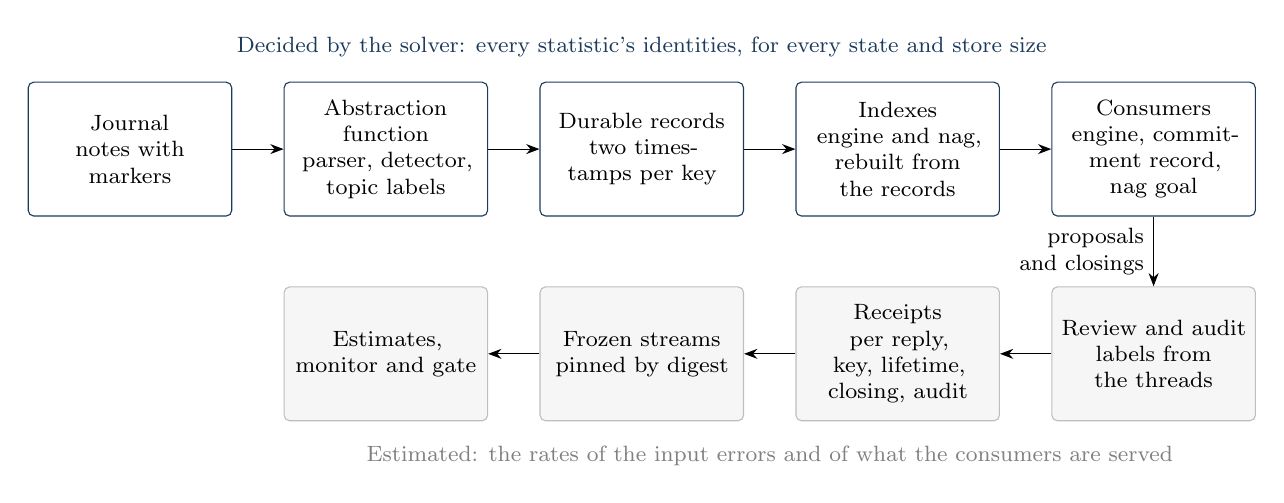
\begin{tikzpicture}[>=Stealth, every node/.style={font=\footnotesize},
  box/.style={draw=dcblue, rounded corners=2pt, align=center, minimum height=1.7cm,
              text width=2.35cm, fill=white},
  soft/.style={draw=dcrule, rounded corners=2pt, align=center, minimum height=1.7cm,
              text width=2.35cm, fill=dcgray}]
\node[box] (j) at (0,0) {Journal\\ notes with markers};
\node[box] (f) at (3.25,0) {Abstraction function\\ parser, detector, topic labels};
\node[box] (r) at (6.5,0) {Durable records\\ two timestamps per key};
\node[box] (i) at (9.75,0) {Indexes\\ engine and nag, rebuilt from the records};
\node[box] (c) at (13,0) {Consumers\\ engine, commitment record, nag goal};
\draw[->] (j) -- (f);
\draw[->] (f) -- (r);
\draw[->] (r) -- (i);
\draw[->] (i) -- (c);
\node[soft] (v) at (13,-2.6) {Review and audit\\ labels from the threads};
\node[soft] (u) at (9.75,-2.6) {Receipts\\ per reply, key, lifetime, closing, audit};
\node[soft] (s) at (6.5,-2.6) {Frozen streams\\ pinned by digest};
\node[soft] (g) at (3.25,-2.6) {Estimates, monitor and gate};
\draw[->] (c) -- node[left, align=right] {proposals\\ and closings} (v);
\draw[->] (v) -- (u);
\draw[->] (u) -- (s);
\draw[->] (s) -- (g);
\node[text=dcblue] at (6.5,1.3) {Decided by the solver: every statistic's identities, for every state
and store size};
\node[text=gray] at (8.125,-3.9) {Estimated: the rates of the input errors and of what the consumers
are served};
\end{tikzpicture}
\caption{The open-item store. The upper row holds the declared objects, whose claims are checked by
a solver; the lower row holds the receipts, from which the rates the declarations cannot reach are
estimated.}\label{fig:store}
\end{figure}

\subsection{Conformance replay}\label{sec:replay}

The verdicts of \cref{tab:store} are about declarations. Whether the simulated designs behave as
the declarations say is a separate question, which Part I answers by replaying recorded events
through the code and through the declared machine \cite[Section~3.4]{part1}. The oracle does this
for the whole deployment, starting from the frozen journal. It reads the journal through its own
implementation of the abstraction function described above and checks that the result is the
simulation's $1{,}362$ keys, with their creation times and the times from which they are closed. It
then steps the module's item machine, the event statistic, the joint statistic and the nag index
through each key's history, evaluating the module's maps as the reference evaluator reads them. At
every daily cycle at which the key was at most seven days old, it compares what the statistics
decide, and what the module's window view shows, with the decisions of the two simulated designs.
All $8{,}966$ decisions agree, and at every cycle the code of each statistic equals the encoding of
the replayed item, which is identity (U) observed on the data.

The replay covers every decision of this corpus, so no sampling bound is needed for it. Both sides
of the comparison receive the same events once the journal has been abstracted, so the replay tests
the designs' code against the module's maps. It does not test the abstraction function itself: the
parser, the detector and the topic labeler reach the claims of this example only through the
receipts of the next section.
\section{Receipts and streams}\label{sec:receipts}

Steps~5 and~6 of the protocol record receipts and freeze them. The protocol asked for one receipt
per suggestion, carrying the item's status from events, the certificate it cites and the reviewer's
label, and for a random sample of items a record of whether the detector found the closing reply
\cite[Section~9]{part2}. The example keeps the random audit as the protocol describes it. It
replaces the receipts per suggestion by receipts at other units, for the reason the next subsection
gives.

\subsection{Why single proposals are the wrong unit}\label{sec:units}

The engine proposes an open item at every cycle until the item is closed or older than seven days.
A reply that the detector misses therefore produces a stale proposal at every cycle from the reply
to the item's seventh day, so one input error yields a run of labels. Kofi's item of
\cref{tab:journal} was proposed at the cycles of days~19 to~24, and the last two proposals were
stale, because the reply of day~22 had been missed. In the gate window the event design logged
$1{,}952$ proposals, of which the review labeled $39$ stale and $30$ duplicate. The $39$ stale labels
came from $7$ keys, two of them stale on seven consecutive days, and the $30$ duplicate labels from
$5$ keys.

Part II estimates rates with a mixture confidence sequence, in the line that begins with Robbins
\cite{robbins} and whose general theory Howard and coauthors give \cite{howard}. Read as an estimate
of a rate, its interval assumes that every observation has one common conditional rate given the
ones before it \cite[Section~5.1]{part2}. Labels that come in runs from one key break that
assumption: once a key has been proposed stale, its next proposal is stale too unless the key ages
out, so an interval computed from the $1{,}952$ labels as if they shared one rate would be too narrow.
A one-sided claim, that the rate is below a target, needs no common rate: by Part II's
Proposition~5.1 it holds for the average, over the observations, of each one's conditional
probability given those before it \cite[Proposition~5.1]{part2}. Even so, the proposals are the
wrong unit for the gate's claims, because that average counts a missed reply once for every day its
item stays young, and the number of days depends on the log-only policy. Once the engine is live, an
answer of ``already handled'' closes the item at its first stale proposal, so a rate per logged
proposal does not carry over to the live engine. The per-proposal labels are kept, as the frozen
stream \code{proposals}, and this text quotes them only as descriptions. For comparison, the window
design logged $3{,}752$ proposals in the same four weeks, of which $1{,}839$ were stale.

Kofi's two stale proposals become one observation at the unit used below. His reply produced a
single reply receipt, released at the cycle of day~23 and labeled stale, and it was one of the
receipts that raised the alarm of Section~\ref{sec:sr}.

\subsection{Step 5: five units of receipt}\label{sec:fiveunits}

Each receipt below has one row per unit, written at a moment fixed in advance, with labels that the
unit's own events decide. \Cref{tab:units} summarizes them.

\begin{table}[ht]
\centering\small
\begin{tabularx}{\textwidth}{>{\raggedright\arraybackslash}p{3.0cm}>{\raggedright\arraybackslash}p{4.2cm}X>{\raggedleft\arraybackslash}p{0.9cm}}
\toprule
Stream & One row per & Labels & Rows\\
\midrule
\code{RepliesGate} & reply to an item at most seven days old, at the next cycle & \code{stale}:
the event design proposes the item at that cycle & $436$\\
\code{KeysGate} & key, at its first proposal & \code{duplicate}: another key holds the same
question & $453$\\
\code{LivesGate} & key whose daily decisions all fall in the window, when its seven days end &
\code{window\_bad}, \code{event\_bad}: the design erred on the key at some cycle & $482$\\
\code{ClosuresGate} & key, at the first cycle after its first closing & \code{spurious}: no reply
had arrived by the time of the closing note & $451$\\
\code{AuditRepliesGate} & audited item with a reply by age four & \code{missed}: memory shows it
open & $140$\\
\code{AuditOpenGate} & audited item without a reply by age four & \code{false\_close}: memory
shows it closed & $76$\\
\bottomrule
\end{tabularx}
\caption{The receipts of the gate window, released on days $28$ to $55$.}\label{tab:units}
\end{table}

A \emph{reply receipt} is written for each reply to an item at most seven days old, at the first
cycle after the reply, and labeled stale when the event design proposes the item at that cycle. For
the event design a reply receipt is stale exactly when memory knows of no closing note for the item
by the time of the cycle: the detector missed the reply, and no other note closed the item first.
The receipt is therefore a measurement, reply by reply, of the detector's misses as the engine
experiences them, and its population, the replies, is the same whether or not the engine's
proposals reach the prompt. The gate's claims about these receipts are one-sided, so they rest on
Part II's Proposition~5.1 and need neither a common rate nor independence between receipts: the
claim is about the average, over the replies, of each reply's probability of a stale receipt given
the receipts before it. Under a fixed parser that probability is the detector's miss rate, slightly
lowered for the replies that a spurious note had closed first. Over the
eight weeks $955$ replies arrived and $916$ reply receipts were written: $31$ replies came to items
that were past seven days at the next cycle, which the engine no longer proposes, and $8$ came after
the last cycle, later on day~55. The streams \code{Replies}, \code{RepliesBefore} and
\code{RepliesGate} hold the reply receipts of the whole deployment, of the weeks before the update
and of the gate window.

The receipts of a cycle are released together, once the review of that cycle is finished, and in
the order of the replies' times. A missed reply has a receipt only after the reviewer has found it,
so a stream that released each receipt as soon as it existed would put the stale ones last; with the
batch rule the order in which a monitor reads the receipts is fixed by the replies' times, whatever
their labels.

A \emph{key receipt} is written for each key at its first proposal and carries the review's
duplicate label. One paraphrase gives one duplicate key, whatever the number of its proposals.
Tomas's second key, \code{grant-report-1235b}, is an example: the event design proposed it at the
cycles of days~52 to~55, and its key receipt, released on day~52, is one row with the label
duplicate. The $30$ duplicate labels of the gate window come from the five keys that
\code{KeysGate} records as duplicates. A paraphrased key and its original share one question, so
their two rows are not independent; the one-sided claim of the gate does not need them to be.

A \emph{lifetime receipt} is written for each key that is not a duplicate and that at least one
design proposed, when its seven days end. It carries one label per design, which is 1 when the
design erred on the key at some cycle: it proposed the item although the item had been answered,
or it did not propose the item while the item was open and the other design proposed it. The second
clause records a missed follow-up in the only way the log can show one, through the other design's
proposal. The two labels of a row concern the same key at the same cycles, so the rows are pairs,
and Part II's comparison of two policies on the same snapshots applies \cite[Section~5.4]{part2}.
That comparison is a sequential form of McNemar's test for paired proportions \cite{mcnemar}: only
the keys on which exactly one design erred carry information about which design errs more, and the
claim that the window design errs more often is one-sided, so Proposition~5.1 of Part II covers it
as well. The
stream \code{LivesGate} keeps the receipts of the keys whose daily decisions all fall in the gate
window, which are the keys created after the cycle of day~27 whose seven days ended by the cycle of
day~55. A key created earlier would bring decisions from before the window into it, including some
from the days of the regression. An error that both designs make at the same cycle, such as
withholding an item that both see as closed, leaves no trace in these labels; the next unit is the
one that sees it.

A \emph{closure receipt} is written for each key that is not a duplicate at the first cycle after
memory learned of its first closing, and carries the review's label: spurious when no reply had
arrived by the time of the closing note. Under the event design the first closing decides the item
for good, so the closure receipts measure, closing by closing, the false closings that the engine
inherits.

An \emph{audit receipt} is written for each item in the random sample when it reaches the age of
four days. The sample is drawn when the item is created, a third of all items. For an item that had
a reply by then, the label says whether memory still shows it open; for an item without a reply,
whether memory shows it closed. The two kinds go to two streams, because they estimate two
different rates. Both describe memory at the age of four days. An error that arises later is outside
them: with the simulation's delays, about one spurious closing note in fourteen arrives after the
fourth day.

\subsection{Where the labels come from}\label{sec:labels}

In a live deployment the labels have different sources, and each source has something it cannot
see. A reply the detector found is known to memory. A reply it missed becomes known when the
reviewer labels the item's next proposal stale and finds the reply in the thread; the reply receipt
is then written with the reply's time and the label~1. A missed reply that the reviewer also
overlooks produces no receipt at all, so the reply streams undercount misses at the rate at which
the review overlooks them. The random audit is the independent check, since its sample is fixed
before anyone knows how the item will go and the auditor reads the whole thread.

False closings are invisible to the review of proposals, because an item closed by a spurious note
is never proposed by the event design again. The review of closings sees them, since it reads the
thread of every first closing. Ben's question about \code{token-bridge-0288} is the example. The
event design proposed it at the cycle of day~11, before the spurious note arrived that evening, and
never again. The review of closings labeled the note spurious at the cycle of day~12; in the
log-only phase nothing feeds a label back to memory, so the item stayed closed under the event
design.
The window design proposed it again on days~14 to~17, once the note's two days in the window had
passed, and for this item that was the right decision. The item was also in the random sample, and
its audit on day~14, at the age of four days, recorded it as open in the thread and closed in
memory. A false closing is the one failure that the event design makes worse than the window design.
The window design stops counting a closing note after two days, so a false closing costs it at most
two days of proposals, while the event design keeps the closing until someone corrects it.

Over the eight weeks the random audit found one false closing among $159$ audited items without a
reply, and six missed replies among $279$ audited items with one. The review of closings labeled
three first closings spurious: Ben's, and two in the gate window.

\subsection{Step 6: freezing the receipts}\label{sec:freeze}

The simulation writes every receipt to a frozen stream, a JSON file with a schema, a provenance
record and the rows, written once in a fixed byte layout so that its SHA-256 digest is
reproducible. The module \code{WMTMReceipts} declares the ten streams that its requests read, each
with its source and digest, and with the three fields that say what an estimate from it is about:
the population it samples, the rule that selects its rows, and the policy under which the rows
were produced. In a live system the policy field holds the digest of the deployed code and flags;
here it names the phase and the parser version. An estimate does not carry over to another policy
without an argument; Section~\ref{sec:releasegate} gives the arguments for the next release and
shows how a small change to its design would defeat one of them. The reference evaluator refuses a stream whose file does not match its declared
digest, before it counts anything: the oracle sets every stale label of \code{RepliesGate} to zero
in a copy of the bundle, and the request on it returns InvalidInput with no count and no interval. The listing below holds the streams and the monitors, which
Section~\ref{sec:regression} explains. Two further streams, the parsed journal and the proposal log,
are frozen for the conformance replay and for the descriptions above; Appendix~\ref{app:streams}
lists all twelve with their digests.

\begin{lstlisting}[style=mettamod]
(DC.Module WMTMReceipts
  (Profile Stochastic)
  (Use Decisions Laws Families Monitors Estimates)     ; PROPOSED Estimates (Part II)
  ;; one receipt per reply, released at the next cycle: was the item proposed (stale)?
  (Stream Replies (Source "streams/replies.json")
    (Digest "sha256:1f5d10eff762371dffdef5e0be4f940e39366a8fe2c6b9227bb7cdb66c82ca0f")
    (Provenance "simulated: replies to items at most seven days old, days 0-55")
    (Population "replies to items at most seven days old at the next cycle")
    (Selection "one row per reply at the next cycle, after its review, by reply time")
    (Policy "log-only phase; parser v1, v2 from day 21 10:00 to day 24 12:00"))
  (Stream RepliesBefore (Source "streams/replies_before.json")
    (Digest "sha256:3a5629468d68aba06e30587dfc23114cbf4ed6e545e426ed4d77c08caf799703")
    (Provenance "simulated: the reply receipts of days 0-21, before the parser update")
    (Population "replies to items at most seven days old at the next cycle")
    (Selection "the rows of Replies released on days 0-21")
    (Policy "log-only phase; parser v1"))
  (Stream RepliesGate (Source "streams/replies_gate.json")
    (Digest "sha256:39def219d4692915bb2d0ce2680d8a85b5aee69729e5f5c419c5c8beb01a764e")
    (Provenance "simulated: the reply receipts of days 28-55")
    (Population "replies to items at most seven days old at the next cycle")
    (Selection "the rows of Replies released on days 28-55")
    (Policy "log-only phase; parser v1, journal re-parsed on day 24"))
  ;; one receipt per key at its first proposal: the review's duplicate label
  (Stream KeysGate (Source "streams/keys_gate.json")
    (Digest "sha256:fd12fdce6989efac157bd53aff04b5e71b40dc710733fedfba64e8caed1ee5e8")
    (Provenance "simulated: keys first proposed on days 28-55")
    (Population "keys that the event design proposes")
    (Selection "one row per key at its first proposal, days 28-55")
    (Policy "log-only phase; parser v1, journal re-parsed on day 24"))
  ;; one receipt per key at the end of its seven days: did each design decide wrongly?
  (Stream LivesGate (Source "streams/lives_gate.json")
    (Digest "sha256:5eb1f54bf60f047de30f1cdfa4516dcefc3a789df5bac4763cdebe14aaaca801")
    (Provenance "simulated: keys whose daily decisions all fall on days 28-55")
    (Population "keys that are not duplicates and that either design proposed")
    (Selection "one row per key whose decisions all fall on days 28-55")
    (Policy "log-only phase; both designs; parser v1"))
  ;; one receipt per key at its first closing: was the closing note a real reply?
  (Stream ClosuresGate (Source "streams/closures_gate.json")
    (Digest "sha256:b11d52683007c2f3f2c25e367ee66f81e4e3393360e3ae9d297fd699806ff209")
    (Provenance "simulated: first closings learned between the cycles of days 27 and 55")
    (Population "first closings of keys that are not duplicates")
    (Selection "one row per key at the cycle after memory learns its first closing")
    (Policy "log-only phase; parser v1, journal re-parsed on day 24"))
  ;; the random audit at age four days, and the targeted audit after the alarm
  (Stream AuditRepliesGate (Source "streams/audit_replies_gate.json")
    (Digest "sha256:8f9a06bed6d5b60ee2007dde3cafd41ff198a57cdc572d7baa59251bf63b97ec")
    (Provenance "simulated: audited items with a reply by age four, days 28-55")
    (Population "items, sampled at creation with probability 1/3")
    (Selection "one row per sampled item replied by age four, audited at four")
    (Policy "log-only phase; parser v1, journal re-parsed on day 24"))
  (Stream AuditOpenGate (Source "streams/audit_open_gate.json")
    (Digest "sha256:840aff688d32968a5d7d2d9c15fc132ca416d109418f260686803037267e8db5")
    (Provenance "simulated: audited items without a reply by age four, days 28-55")
    (Population "items, sampled at creation with probability 1/3")
    (Selection "one row per sampled item not replied by age four, audited at four")
    (Policy "log-only phase; parser v1, journal re-parsed on day 24"))
  (Stream AuditAfterAlarm (Source "streams/audit_after_alarm.json")
    (Digest "sha256:5d6f7667bbdf76e094d5827d64beb8b36b1c5f959b40af405d1844c743d6b0fc")
    (Provenance "simulated: audited replies received after the receipts of the alarm")
    (Population "replies received from the alarm cycle to the audit on day 24")
    (Selection "every such reply, audited on day 24 at 09:00")
    (Policy "log-only phase; parser v2"))
  (Stream AuditV2 (Source "streams/audit_replies_v2.json")
    (Digest "sha256:ea80e318024f8534248b4d58a075b9243dfc1ad6dfa71d842a7bd74bfbef0038")
    (Provenance "simulated: every reply between the parser update and the audit")
    (Population "replies received from the parser update to the audit on day 24")
    (Selection "every such reply, audited on day 24 at 09:00")
    (Policy "log-only phase; parser v2"))

  ;; the monitors: a missed reply that reaches a proposal, accepted at one in twenty
  (Carrier One  (Of Symbol) (Enum one))
  (Carrier Rate (Of Symbol) (Enum accepted tenth fifth twofifths))
  (Map miss-rate (From Rate) (To Rational01)
    (Table (accepted (Rat 1 20)) (tenth (Rat 1 10)) (fifth (Rat 1 5))
           (twofifths (Rat 2 5))))
  (Map stale (Parameters ($r Rate)) (From One) (To (Law Nat))
    (Body ($u) (Coin (miss-rate $r))))
  (Monitor MissTenth (Context One) (Null (stale accepted)) (Alternative (stale tenth))
    (Columns (observation "stale")))
  (Monitor MissFifth (Context One) (Null (stale accepted)) (Alternative (stale fifth))
    (Columns (observation "stale")))
  (Monitor MissTwoFifths (Context One) (Null (stale accepted))
    (Alternative (stale twofifths)) (Columns (observation "stale"))))
\end{lstlisting}

The gate reads the receipts released on days~28 to~55, a window fixed before it began, and the
regression of the fourth week lies outside every stream it reads. The reply, key and closure
receipts of the window concern replies, proposals and closings after the cycle of day~27. The
audits of the window concern items created from day~24 on, whose replies were all parsed by
version~1, at the latest by the re-parse at noon on day~24. The lifetime receipts are restricted,
as described above, to keys created after the cycle of day~27.
\section{The regression}\label{sec:regression}

Step~8 of the protocol runs a mixture monitor on the stale rate. In the calendar it comes first,
since the monitor reads the reply receipts from day~0, and it is the step that met the one incident
of the eight weeks.

\subsection{Step 8: the monitors}\label{sec:monitors}

The team accepts a stale reply receipt rate of one in twenty. Parts~I and~II stated that rate per
suggestion; the example states it per reply, the unit at which it can be estimated
(Section~\ref{sec:units}). Once the engine is live and an answer of ``already handled'' closes the
item, each stale reply receipt costs one stale proposal, and in the gate window there were about
four proposals for every reply receipt, so one in twenty per reply is the stricter of the two
targets. The module declares three monitors, each comparing the accepted rate with one failing
rate, $1/10$, $1/5$ or $2/5$, as Part II's Pattern~8 did \cite[Section~6.8]{part2}. For a receipt
with label $X_n$ and an alternative rate $q$ against the accepted rate $p_0=1/20$, a monitor's
factor is the likelihood ratio
\[
L_n=\left(\frac{q}{p_0}\right)^{X_n}\left(\frac{1-q}{1-p_0}\right)^{1-X_n},
\]
which exceeds one for a stale receipt and falls short of one otherwise. The requests:

\begin{lstlisting}[style=mettamod]
!(dc.run WMTMReceipts (CheckMonitor MissTenth))
!(dc.run WMTMReceipts (CheckMonitor MissFifth))
!(dc.run WMTMReceipts (CheckMonitor MissTwoFifths))
!(dc.run WMTMReceipts
   (Detect MissTenth MissFifth MissTwoFifths (On Replies) (Level (Rat 1 100))
           (Combine Mixture)))
!(dc.run WMTMReceipts
   (Detect MissTenth MissFifth MissTwoFifths (On Replies) (Combine Mixture)
           (Scheme ShiryaevRoberts) (MeanTimeToFalseAlarm 100000)))   ; PROPOSED Scheme
!(dc.run WMTMReceipts
   (EstimateRate (On RepliesBefore) (Column "stale") (Equals 1) (Level (Rat 1 100))))
!(dc.run WMTMReceipts
   (EstimateRate (On AuditAfterAlarm) (Column "missed") (Equals 1) (Level (Rat 1 100))))
!(dc.run WMTMReceipts
   (EstimateRate (On AuditV2) (Column "missed") (Equals 1) (Level (Rat 1 100))))
\end{lstlisting}

A monitor declares the context in which each observation is made, and these three have a single
context, the value \code{one} of the carrier \code{One}. \code{CheckMonitor} is therefore one
identity for each monitor, and it is Checked for all three by exact arithmetic, without a solver:
under the accepted rate the factor's expectation is exactly one. The two \code{Detect} requests combine the three monitors as a mixture
and differ in how they accumulate evidence. The first is Part II's scheme, which the patch calls
\code{Ville}: each monitor multiplies its factors from the first receipt on, the mixture averages
the three products, and the alarm is raised when the average reaches $1/\alpha=100$. Ville's
inequality bounds the probability of ever raising a false alarm by $\alpha=0.01$, however long the
monitor runs \cite{ville,ramdas}. This $\alpha$ is the \emph{level} of the guarantee, the
probability of error it allows, and every estimate in this example is stated at the same level: an
interval at level $0.01$ fails to contain the true rate with probability at most $0.01$. The second
\code{Detect} request is the changepoint scheme of Section~\ref{sec:sr}, which the deployment ran in
the loop. The remaining requests are the estimates of Section~\ref{sec:confirm}.

\subsection{What happened}\label{sec:happened}

Parser version~2 went live on day~21, a Monday, at 10:00. It changed how the reply detector matched
a ``decided:'' note to an open item, and in the simulation it misses a reply with probability
$1/4$, against $0.015$ for version~1. Nothing in the declarations changed. The detector is part of
the abstraction function, outside every declaration, and the statistics went on answering correctly
for the events they were given, so the change showed only in the receipts. Receipt~$362$ was the
last for a reply received before the update; of the $37$ receipts from receipt~$363$ to
receipt~$399$, released at the cycles of days~22 and~23, ten were stale.

\subsection{Why a monitor started at the first receipt stays silent}\label{sec:debt}

Part II's monitor never fired. Its value after the first receipt, $0.807$, was the largest it
reached over the whole stream. By receipt~$362$ the logarithm of its value had fallen to $-16.93$;
the alarm needs the logarithm to reach $\ln 100=4.61$; and by receipt~$399$, after the ten stale
receipts, it stood at $-11.46$. After the rollback it fell again, to $-31.2$ at the last of the
$916$ receipts.

Each receipt that is not stale multiplies every monitor's product by $(1-q)/(1-p_0)<1$, so three
healthy weeks leave every product, and hence their average, far below one. A change that comes
after them must first make up that factor before the monitor can count any evidence against the
accepted rate. The monitor answers the question it was built for, whether the stream since the
first receipt is consistent with the accepted rate, and after $362$ healthy receipts a few dozen
bad ones take a long time to change that answer. Part II's simulations of monitors used streams
whose rate was the same from the first receipt on \cite[Section~5.5]{part2}, where this does not
arise.

A counterfactual run of the same simulation without the rollback shows the cost. With version~2
left in place, Part II's monitor would have fired at receipt~$524$ on day~30, a week after the
changepoint monitor. On days~24 to~30 the event design would have logged $169$ stale proposals,
where the run with the rollback logged $21$: the late alarm would have cost $148$ stale proposals.

\subsection{A changepoint monitor}\label{sec:sr}

The statistics of quickest detection address this case: observations follow one law until an
unknown time and another afterwards, and an alarm should come soon after the change and rarely
before it. Page's cumulative sum \cite{page} and the procedure of Shiryaev and Roberts
\cite{shiryaev,roberts} are the classical answers, with optimality results by Lorden \cite{lorden}
and Pollak \cite{pollak}. Shin, Ramdas and Rinaldo built such procedures from e-processes,
nonnegative processes whose expected value under the null hypothesis is at most one at every
stopping time \cite{shin}. That construction extends them to composite null hypotheses, which allow
a range of rates, such as ``the rate is at most $p_0$'', instead of a single one. The example uses
the Shiryaev--Roberts form. For each alternative $q$, let $R_0=0$ and
\[
R_n=(1+R_{n-1})\,L_n,\qquad\text{equivalently}\qquad
R_n=\sum_{k=1}^{n}\ \prod_{j=k}^{n}L_j .
\]
The term for $k$ is the likelihood ratio of ``the rate became $q$ at receipt $k$'' against ``no
change'', over the receipts from $k$ to $n$, so $R_n$ adds the evidence for every possible start of
a change. The term for $k=1$ is the product of Part II's monitor. The mixture $\bar R_n$ averages
$R_n$ over the three alternatives, and the alarm is raised at the first $n$ with $\bar R_n\ge A$.

\begin{proposition}[False alarms of the changepoint monitor]\label{prop:sr}
Let $X_1,X_2,\ldots$ be binary labels such that, for every $n$, the conditional probability that
$X_n=1$ given $X_1,\ldots,X_{n-1}$ is at most $p_0$. Let $q_1,\ldots,q_m>p_0$, let $R^{(i)}_n$ be the
statistic above for $q_i$, $\bar R_n$ their average, and $T$ the first $n$ with $\bar R_n\ge A$,
for some $A>0$. Then
\begin{enumerate}
\item $\mathbb E[T]\ge A$, and
\item $P(T\le N)\le N/A$ for every $N\ge 1$.
\end{enumerate}
\end{proposition}

\begin{proof}
Write $p_n$ for the conditional probability that $X_n=1$ given the past. The conditional expectation
of the factor for $q_i$ is $p_nq_i/p_0+(1-p_n)(1-q_i)/(1-p_0)$, which increases with $p_n$ because
$q_i>p_0$ and equals one at $p_n=p_0$, so it is at most one. Hence the conditional expectation of
$R^{(i)}_n$ is at most $1+R^{(i)}_{n-1}$, and the same holds for the average: the conditional
expectation of $\bar R_n$ is at most $1+\bar R_{n-1}$.

For the first part, $\bar R_n-n$ is then a supermartingale that starts at zero: its conditional
expectation, given the past, never exceeds its last value. For every $k$ the stopping time
$T\wedge k$ is bounded, and optional stopping gives $\mathbb E[\bar R_{T\wedge k}]\le\mathbb
E[T\wedge k]$. Since $\bar R$ is nonnegative and at least $A$ at time $T$, the left side is at least
$A\,P(T\le k)$. Letting $k$ grow gives $\mathbb E[T]\ge A\,P(T<\infty)$. If $P(T<\infty)=1$ this
is the claim, and otherwise $\mathbb E[T]$ is infinite; hence $\mathbb E[T]\ge A$.

For the second part, fix $N$ and let $M_n=\bar R_n+(N-n)$ for $n=0,\ldots,N$. Then $M_0=N$, every
$M_n$ is nonnegative, and the conditional expectation of $M_n$ is at most $1+\bar R_{n-1}+N-n=
M_{n-1}$, so $M$ is a nonnegative supermartingale. Ville's inequality bounds the probability that
it ever reaches $A$ by $M_0/A=N/A$. On the event $T\le N$, $M_T\ge\bar R_T\ge A$. Hence $P(T\le
N)\le N/A$.
\end{proof}

\plain A monitor that adds up the evidence for a change starting at every possible receipt will
raise a false alarm sooner or later, but not soon. With the threshold at $100{,}000$, it reads at
least $100{,}000$ receipts on average before its first false alarm when nothing has changed, and the
chance of a false alarm within any $N$ receipts is at most $N$ in $100{,}000$.

The guarantee is of a different kind from Ville's. Ville's inequality bounds the probability of any
false alarm over an unbounded future. The proposition bounds the expected number of receipts before
a false alarm, and its probability over any fixed number of receipts, but not over an unbounded
future: if each receipt is stale with some positive probability, independently of the others, the
stream contains, with probability one, a run of stale receipts long enough to carry $\bar R_n$ past
any threshold. The ability to detect a late change is paid for with false alarms at long intervals,
at least $A$ receipts apart on average if the monitor restarts after each. An alarm is then a
reason to look, and the look has to produce evidence that the alarm did not use, which is what the
confirmation rule of Section~\ref{sec:confirm} requires. The deployment set $A=100{,}000$. At $16.4$
receipts a day that is at least $16.7$ years of receipts, on average, before a false alarm. By the
second part, the probability of a false alarm was at most $0.0092$ over the $916$ receipts of the
eight weeks, and it is at most $0.06$ over a year of receipts at the same rate. The detection delay
of such procedures grows only with the logarithm of $A$ \cite{lorden,pollak}. Declaring this
monitor needs two new arguments of \code{Detect}, the scheme and the mean time to a false alarm,
which the registry patch of Appendix~\ref{app:registry} adds.

At the cycle of day~23 the monitor read the receipts released that morning, and at receipt~$399$
the mixture reached $116{,}558$, whose logarithm $11.67$ exceeds $\ln 100{,}000=11.51$. The alarm
came $47$ hours after the update; at the update the logarithm of the mixture had been $2.12$. The
monitor stopped at its alarm, so receipts~$400$ to~$419$, the rest of that morning's batch and the
batch of day~24, were read by no monitor. \Cref{fig:monitors} shows the two monitors on the whole
stream.

\pgfplotstableread[row sep=\\]{receipt ville loop\\
1 -0.2144 -0.2144\\
2 -0.4027 0.3890\\
3 -0.5684 0.7139\\
4 -0.7150 0.9287\\
5 -0.8462 1.0853\\
6 -0.9649 1.2063\\
7 -1.0736 1.3037\\
8 -1.1743 1.3843\\
9 -1.2686 1.4524\\
10 -1.3577 1.5108\\
11 -1.4424 1.5617\\
12 -1.5235 1.6064\\
13 -1.6015 1.6460\\
14 -1.6768 1.6815\\
15 -1.7499 1.7133\\
16 -1.8210 1.7420\\
17 -1.8902 1.7682\\
18 -1.9579 1.7920\\
19 -2.0241 1.8137\\
20 -2.0891 1.8337\\
21 -2.1529 1.8521\\
22 -2.2157 1.8691\\
23 -2.2776 1.8848\\
24 -2.3387 1.8993\\
25 -2.3990 1.9128\\
26 -2.4586 1.9254\\
27 -2.5177 1.9371\\
28 -2.5762 1.9480\\
29 -2.6342 1.9581\\
30 -2.6918 1.9677\\
31 -2.7491 1.9766\\
32 -2.8059 1.9849\\
33 -2.8625 1.9927\\
34 -2.9188 2.0001\\
35 -2.9749 2.0069\\
36 -3.0307 2.0134\\
37 -3.0864 2.0195\\
38 -3.1418 2.0252\\
39 -3.1972 2.0306\\
40 -3.2523 2.0357\\
41 -3.3074 2.0404\\
42 -3.3624 2.0449\\
43 -3.4172 2.0492\\
44 -3.4720 2.0531\\
45 -3.5267 2.0569\\
46 -3.5813 2.0605\\
47 -3.6358 2.0638\\
48 -3.6903 2.0670\\
49 -3.7448 2.0700\\
50 -3.7992 2.0728\\
51 -3.8536 2.0755\\
52 -3.9079 2.0780\\
53 -3.9622 2.0804\\
54 -4.0165 2.0826\\
55 -4.0708 2.0847\\
56 -4.1250 2.0867\\
57 -4.1792 2.0886\\
58 -4.2334 2.0904\\
59 -4.2876 2.0921\\
60 -4.3418 2.0937\\
61 -4.3960 2.0952\\
62 -4.4501 2.0967\\
63 -4.5042 2.0980\\
64 -4.5584 2.0993\\
65 -4.6125 2.1005\\
66 -4.6666 2.1017\\
67 -4.7207 2.1028\\
68 -4.7749 2.1038\\
69 -4.8290 2.1048\\
70 -4.8831 2.1057\\
71 -4.9372 2.1066\\
72 -4.9912 2.1074\\
73 -5.0453 2.1082\\
74 -5.0994 2.1089\\
75 -5.1535 2.1096\\
76 -5.2076 2.1103\\
77 -5.2617 2.1109\\
78 -5.3158 2.1115\\
79 -5.3698 2.1121\\
80 -5.4239 2.1126\\
81 -5.4780 2.1131\\
82 -5.5321 2.1136\\
83 -5.5861 2.1141\\
84 -5.6402 2.1145\\
85 -5.6943 2.1149\\
86 -5.7484 2.1153\\
87 -5.8024 2.1156\\
88 -5.8565 2.1160\\
89 -5.9106 2.1163\\
90 -5.9646 2.1166\\
91 -6.0187 2.1169\\
92 -6.0728 2.1172\\
93 -6.1268 2.1174\\
94 -6.1809 2.1177\\
95 -5.4878 3.3420\\
96 -5.5418 3.1954\\
97 -5.5959 3.0751\\
98 -5.6500 2.9763\\
99 -5.7040 2.8944\\
100 -5.7581 2.8257\\
101 -5.8122 2.7673\\
102 -5.8662 2.7169\\
103 -5.9203 2.6729\\
104 -5.2272 3.8066\\
105 -5.2812 3.6668\\
106 -5.3353 3.5473\\
107 -5.3894 3.4442\\
108 -5.4434 3.3545\\
109 -4.7503 4.5004\\
110 -4.8043 4.3423\\
111 -4.8584 4.2036\\
112 -4.9125 4.0811\\
113 -4.9665 3.9717\\
114 -5.0206 3.8731\\
115 -5.0747 3.7834\\
116 -5.1288 3.7011\\
117 -5.1828 3.6249\\
118 -5.2369 3.5541\\
119 -5.2910 3.4879\\
120 -4.5978 4.5017\\
121 -4.6519 4.3831\\
122 -4.7059 4.2764\\
123 -4.7600 4.1793\\
124 -4.8141 4.0901\\
125 -4.8681 4.0075\\
126 -4.9222 3.9303\\
127 -4.9763 3.8579\\
128 -5.0304 3.7896\\
129 -5.0844 3.7248\\
130 -5.1385 3.6633\\
131 -5.1926 3.6047\\
132 -5.2466 3.5487\\
133 -5.3007 3.4952\\
134 -5.3548 3.4439\\
135 -5.4088 3.3946\\
136 -5.4629 3.3473\\
137 -5.5170 3.3017\\
138 -5.5710 3.2579\\
139 -5.6251 3.2156\\
140 -5.6792 3.1748\\
141 -5.7332 3.1354\\
142 -5.7873 3.0973\\
143 -5.8414 3.0605\\
144 -5.8954 3.0249\\
145 -5.9495 2.9905\\
146 -6.0036 2.9572\\
147 -6.0576 2.9249\\
148 -6.1117 2.8937\\
149 -6.1658 2.8635\\
150 -6.2198 2.8343\\
151 -6.2739 2.8060\\
152 -6.3280 2.7786\\
153 -6.3820 2.7521\\
154 -6.4361 2.7264\\
155 -6.4902 2.7016\\
156 -6.5442 2.6777\\
157 -6.5983 2.6545\\
158 -6.6524 2.6322\\
159 -6.7064 2.6106\\
160 -6.7605 2.5897\\
161 -6.8146 2.5696\\
162 -6.8686 2.5502\\
163 -6.9227 2.5315\\
164 -6.9768 2.5135\\
165 -7.0308 2.4962\\
166 -7.0849 2.4795\\
167 -7.1390 2.4635\\
168 -7.1930 2.4481\\
169 -7.2471 2.4332\\
170 -7.3012 2.4190\\
171 -7.3552 2.4053\\
172 -7.4093 2.3922\\
173 -7.4634 2.3796\\
174 -7.5175 2.3676\\
175 -7.5715 2.3560\\
176 -7.6256 2.3450\\
177 -7.6797 2.3344\\
178 -7.7337 2.3243\\
179 -7.7878 2.3146\\
180 -7.8419 2.3053\\
181 -7.8959 2.2964\\
182 -7.9500 2.2880\\
183 -8.0041 2.2799\\
184 -8.0581 2.2722\\
185 -8.1122 2.2648\\
186 -8.1663 2.2578\\
187 -8.2203 2.2511\\
188 -8.2744 2.2447\\
189 -8.3285 2.2386\\
190 -8.3825 2.2328\\
191 -8.4366 2.2273\\
192 -8.4907 2.2220\\
193 -8.5447 2.2170\\
194 -8.5988 2.2122\\
195 -8.6529 2.2077\\
196 -8.7069 2.2034\\
197 -8.7610 2.1992\\
198 -8.8151 2.1953\\
199 -8.8691 2.1916\\
200 -8.9232 2.1881\\
201 -8.9773 2.1847\\
202 -9.0313 2.1815\\
203 -9.0854 2.1785\\
204 -9.1395 2.1756\\
205 -9.1935 2.1728\\
206 -9.2476 2.1702\\
207 -9.3017 2.1678\\
208 -9.3557 2.1654\\
209 -9.4098 2.1632\\
210 -9.4639 2.1611\\
211 -9.5179 2.1591\\
212 -9.5720 2.1572\\
213 -9.6261 2.1553\\
214 -9.6801 2.1536\\
215 -9.7342 2.1520\\
216 -9.7883 2.1504\\
217 -9.8423 2.1490\\
218 -9.8964 2.1476\\
219 -9.9505 2.1463\\
220 -10.0045 2.1450\\
221 -10.0586 2.1438\\
222 -10.1127 2.1427\\
223 -10.1667 2.1416\\
224 -10.2208 2.1406\\
225 -9.5277 3.3555\\
226 -9.5817 3.2102\\
227 -9.6358 3.0910\\
228 -9.6899 2.9929\\
229 -9.7439 2.9114\\
230 -9.7980 2.8430\\
231 -9.8521 2.7846\\
232 -9.9061 2.7342\\
233 -9.9602 2.6900\\
234 -10.0143 2.6507\\
235 -10.0683 2.6156\\
236 -10.1224 2.5838\\
237 -10.1765 2.5550\\
238 -10.2305 2.5285\\
239 -10.2846 2.5042\\
240 -10.3387 2.4818\\
241 -10.3927 2.4611\\
242 -10.4468 2.4418\\
243 -10.5009 2.4239\\
244 -10.5549 2.4072\\
245 -10.6090 2.3916\\
246 -10.6631 2.3769\\
247 -10.7171 2.3632\\
248 -10.7712 2.3504\\
249 -10.8253 2.3383\\
250 -10.8793 2.3269\\
251 -10.9334 2.3161\\
252 -10.9875 2.3060\\
253 -11.0415 2.2965\\
254 -11.0956 2.2874\\
255 -11.1497 2.2789\\
256 -11.2037 2.2708\\
257 -11.2578 2.2631\\
258 -11.3119 2.2559\\
259 -11.3660 2.2490\\
260 -11.4200 2.2425\\
261 -11.4741 2.2364\\
262 -11.5282 2.2305\\
263 -11.5822 2.2250\\
264 -11.6363 2.2197\\
265 -11.6904 2.2147\\
266 -11.7444 2.2100\\
267 -11.7985 2.2055\\
268 -11.8526 2.2012\\
269 -11.9066 2.1971\\
270 -11.9607 2.1933\\
271 -12.0148 2.1896\\
272 -12.0688 2.1862\\
273 -12.1229 2.1829\\
274 -12.1770 2.1797\\
275 -12.2310 2.1768\\
276 -12.2851 2.1740\\
277 -12.3392 2.1713\\
278 -12.3932 2.1687\\
279 -12.4473 2.1663\\
280 -12.5014 2.1641\\
281 -12.5554 2.1619\\
282 -12.6095 2.1598\\
283 -12.6636 2.1579\\
284 -12.7176 2.1560\\
285 -12.7717 2.1543\\
286 -12.8258 2.1526\\
287 -12.8798 2.1510\\
288 -12.9339 2.1495\\
289 -12.9880 2.1481\\
290 -13.0420 2.1467\\
291 -13.0961 2.1455\\
292 -13.1502 2.1443\\
293 -13.2042 2.1431\\
294 -13.2583 2.1420\\
295 -13.3124 2.1410\\
296 -13.3664 2.1400\\
297 -13.4205 2.1391\\
298 -13.4746 2.1382\\
299 -13.5286 2.1373\\
300 -13.5827 2.1366\\
301 -13.6368 2.1358\\
302 -13.6908 2.1351\\
303 -13.7449 2.1344\\
304 -13.7990 2.1338\\
305 -13.8530 2.1332\\
306 -13.9071 2.1326\\
307 -13.9612 2.1320\\
308 -14.0152 2.1315\\
309 -14.0693 2.1310\\
310 -14.1234 2.1306\\
311 -14.1774 2.1301\\
312 -14.2315 2.1297\\
313 -14.2856 2.1293\\
314 -14.3396 2.1289\\
315 -14.3937 2.1286\\
316 -14.4478 2.1282\\
317 -14.5018 2.1279\\
318 -14.5559 2.1276\\
319 -14.6100 2.1273\\
320 -14.6641 2.1271\\
321 -14.7181 2.1268\\
322 -14.7722 2.1266\\
323 -14.8263 2.1263\\
324 -14.8803 2.1261\\
325 -14.9344 2.1259\\
326 -14.9885 2.1257\\
327 -15.0425 2.1255\\
328 -15.0966 2.1253\\
329 -15.1507 2.1252\\
330 -15.2047 2.1250\\
331 -15.2588 2.1249\\
332 -15.3129 2.1247\\
333 -15.3669 2.1246\\
334 -15.4210 2.1245\\
335 -15.4751 2.1243\\
336 -15.5291 2.1242\\
337 -15.5832 2.1241\\
338 -15.6373 2.1240\\
339 -15.6913 2.1239\\
340 -15.7454 2.1238\\
341 -15.7995 2.1237\\
342 -15.8535 2.1237\\
343 -15.9076 2.1236\\
344 -15.9617 2.1235\\
345 -16.0157 2.1234\\
346 -16.0698 2.1234\\
347 -16.1239 2.1233\\
348 -16.1779 2.1232\\
349 -16.2320 2.1232\\
350 -16.2861 2.1231\\
351 -16.3401 2.1231\\
352 -16.3942 2.1230\\
353 -16.4483 2.1230\\
354 -16.5023 2.1229\\
355 -16.5564 2.1229\\
356 -16.6105 2.1229\\
357 -16.6645 2.1228\\
358 -16.7186 2.1228\\
359 -16.7727 2.1228\\
360 -16.8267 2.1227\\
361 -16.8808 2.1227\\
362 -16.9349 2.1227\\
363 -16.2417 3.3449\\
364 -16.2958 3.1986\\
365 -16.3499 3.0786\\
366 -16.4039 2.9799\\
367 -16.4580 2.8981\\
368 -16.5121 2.8295\\
369 -16.5661 2.7711\\
370 -15.8730 3.9298\\
371 -15.9271 3.7792\\
372 -15.9811 3.6500\\
373 -16.0352 3.5385\\
374 -16.0893 3.4413\\
375 -16.1433 3.3556\\
376 -16.1974 3.2792\\
377 -16.2515 3.2103\\
378 -16.3055 3.1477\\
379 -15.6124 4.2184\\
380 -15.6664 4.0879\\
381 -15.7205 3.9730\\
382 -15.7746 3.8706\\
383 -15.0814 4.9989\\
384 -14.3883 6.3574\\
385 -14.4423 6.1245\\
386 -13.7492 7.6551\\
387 -13.8033 7.3704\\
388 -13.1101 9.0476\\
389 -13.1642 8.7189\\
390 -13.2183 8.4142\\
391 -13.2723 8.1338\\
392 -13.3264 7.8770\\
393 -13.3805 7.6426\\
394 -13.4345 7.4282\\
395 -13.4886 7.2315\\
396 -12.7954 8.6587\\
397 -12.8495 8.4263\\
398 -12.1564 9.9673\\
399 -11.4632 11.6661\\
400 -10.7701 nan\\
401 -10.8241 nan\\
402 -10.8782 nan\\
403 -10.9323 nan\\
404 -10.9863 nan\\
405 -11.0404 nan\\
406 -10.3473 nan\\
407 -10.4013 nan\\
408 -10.4554 nan\\
409 -9.7622 nan\\
410 -9.0691 nan\\
411 -8.3760 nan\\
412 -8.4300 nan\\
413 -8.4841 nan\\
414 -8.5382 nan\\
415 -8.5922 nan\\
416 -8.6463 nan\\
417 -8.7004 nan\\
418 -8.0072 nan\\
419 -8.0613 nan\\
420 -8.1153 -0.2144\\
421 -8.1694 0.3890\\
422 -8.2235 0.7139\\
423 -8.2775 0.9287\\
424 -8.3316 1.0853\\
425 -8.3857 1.2063\\
426 -8.4397 1.3037\\
427 -8.4938 1.3843\\
428 -7.8007 2.9258\\
429 -7.8547 2.7425\\
430 -7.9088 2.5960\\
431 -7.9629 2.4811\\
432 -8.0169 2.3922\\
433 -8.0710 2.3238\\
434 -8.1251 2.2713\\
435 -8.1791 2.2308\\
436 -8.2332 2.1994\\
437 -8.2873 2.1750\\
438 -8.3413 2.1560\\
439 -8.3954 2.1411\\
440 -8.4495 2.1294\\
441 -8.5035 2.1202\\
442 -8.5576 2.1131\\
443 -8.6117 2.1075\\
444 -8.6657 2.1033\\
445 -8.7198 2.1002\\
446 -8.7739 2.0978\\
447 -8.8279 2.0962\\
448 -8.8820 2.0952\\
449 -8.9361 2.0945\\
450 -8.9901 2.0943\\
451 -9.0442 2.0943\\
452 -9.0983 2.0946\\
453 -9.1523 2.0950\\
454 -9.2064 2.0956\\
455 -9.2605 2.0963\\
456 -9.3145 2.0971\\
457 -9.3686 2.0979\\
458 -9.4227 2.0988\\
459 -9.4768 2.0997\\
460 -9.5308 2.1005\\
461 -9.5849 2.1014\\
462 -9.6390 2.1023\\
463 -9.6930 2.1032\\
464 -9.7471 2.1041\\
465 -9.8012 2.1049\\
466 -9.8552 2.1057\\
467 -9.9093 2.1065\\
468 -9.9634 2.1072\\
469 -10.0174 2.1080\\
470 -10.0715 2.1087\\
471 -10.1256 2.1093\\
472 -10.1796 2.1100\\
473 -10.2337 2.1106\\
474 -10.2878 2.1112\\
475 -10.3418 2.1117\\
476 -10.3959 2.1123\\
477 -10.4500 2.1128\\
478 -10.5040 2.1133\\
479 -10.5581 2.1137\\
480 -10.6122 2.1141\\
481 -10.6662 2.1146\\
482 -10.7203 2.1150\\
483 -10.7744 2.1153\\
484 -10.8284 2.1157\\
485 -10.8825 2.1160\\
486 -10.9366 2.1163\\
487 -10.9906 2.1167\\
488 -11.0447 2.1169\\
489 -11.0988 2.1172\\
490 -11.1528 2.1175\\
491 -11.2069 2.1177\\
492 -11.2610 2.1180\\
493 -11.3150 2.1182\\
494 -11.3691 2.1184\\
495 -11.4232 2.1186\\
496 -11.4772 2.1188\\
497 -11.5313 2.1189\\
498 -11.5854 2.1191\\
499 -11.6394 2.1193\\
500 -11.6935 2.1194\\
501 -11.7476 2.1196\\
502 -11.8016 2.1197\\
503 -11.8557 2.1198\\
504 -11.9098 2.1200\\
505 -11.9638 2.1201\\
506 -12.0179 2.1202\\
507 -12.0720 2.1203\\
508 -12.1260 2.1204\\
509 -12.1801 2.1205\\
510 -12.2342 2.1206\\
511 -12.2882 2.1207\\
512 -12.3423 2.1207\\
513 -12.3964 2.1208\\
514 -12.4504 2.1209\\
515 -12.5045 2.1210\\
516 -12.5586 2.1210\\
517 -12.6126 2.1211\\
518 -12.6667 2.1211\\
519 -12.7208 2.1212\\
520 -12.7749 2.1212\\
521 -12.8289 2.1213\\
522 -12.8830 2.1213\\
523 -12.9371 2.1214\\
524 -12.9911 2.1214\\
525 -13.0452 2.1215\\
526 -13.0993 2.1215\\
527 -13.1533 2.1215\\
528 -13.2074 2.1216\\
529 -13.2615 2.1216\\
530 -13.3155 2.1216\\
531 -13.3696 2.1217\\
532 -13.4237 2.1217\\
533 -13.4777 2.1217\\
534 -13.5318 2.1217\\
535 -13.5859 2.1218\\
536 -13.6399 2.1218\\
537 -13.6940 2.1218\\
538 -13.7481 2.1218\\
539 -13.8021 2.1218\\
540 -13.8562 2.1219\\
541 -13.9103 2.1219\\
542 -13.9643 2.1219\\
543 -14.0184 2.1219\\
544 -14.0725 2.1219\\
545 -14.1265 2.1219\\
546 -14.1806 2.1219\\
547 -14.2347 2.1220\\
548 -14.2887 2.1220\\
549 -14.3428 2.1220\\
550 -14.3969 2.1220\\
551 -14.4509 2.1220\\
552 -14.5050 2.1220\\
553 -14.5591 2.1220\\
554 -14.6131 2.1220\\
555 -14.6672 2.1220\\
556 -14.7213 2.1220\\
557 -14.7753 2.1220\\
558 -14.8294 2.1220\\
559 -14.8835 2.1221\\
560 -14.9375 2.1221\\
561 -14.9916 2.1221\\
562 -15.0457 2.1221\\
563 -15.0997 2.1221\\
564 -15.1538 2.1221\\
565 -15.2079 2.1221\\
566 -15.2619 2.1221\\
567 -15.3160 2.1221\\
568 -15.3701 2.1221\\
569 -15.4241 2.1221\\
570 -15.4782 2.1221\\
571 -15.5323 2.1221\\
572 -15.5863 2.1221\\
573 -15.6404 2.1221\\
574 -15.6945 2.1221\\
575 -15.7485 2.1221\\
576 -15.8026 2.1221\\
577 -15.8567 2.1221\\
578 -15.9107 2.1221\\
579 -15.9648 2.1221\\
580 -16.0189 2.1221\\
581 -16.0730 2.1221\\
582 -16.1270 2.1221\\
583 -16.1811 2.1221\\
584 -16.2352 2.1221\\
585 -16.2892 2.1221\\
586 -16.3433 2.1221\\
587 -16.3974 2.1221\\
588 -16.4514 2.1221\\
589 -16.5055 2.1221\\
590 -15.8123 3.3446\\
591 -15.8664 3.1982\\
592 -15.9205 3.0782\\
593 -15.9745 2.9795\\
594 -16.0286 2.8977\\
595 -16.0827 2.8291\\
596 -16.1367 2.7707\\
597 -16.1908 2.7203\\
598 -15.4977 3.8634\\
599 -15.5517 3.7193\\
600 -15.6058 3.5959\\
601 -15.6599 3.4893\\
602 -15.7139 3.3964\\
603 -15.7680 3.3144\\
604 -15.8221 3.2411\\
605 -15.8761 3.1751\\
606 -15.9302 3.1150\\
607 -15.9843 3.0599\\
608 -16.0383 3.0091\\
609 -16.0924 2.9620\\
610 -16.1465 2.9182\\
611 -16.2005 2.8773\\
612 -16.2546 2.8389\\
613 -16.3087 2.8030\\
614 -16.3627 2.7691\\
615 -16.4168 2.7372\\
616 -16.4709 2.7072\\
617 -16.5249 2.6787\\
618 -16.5790 2.6518\\
619 -16.6331 2.6263\\
620 -16.6871 2.6022\\
621 -16.7412 2.5792\\
622 -16.7953 2.5574\\
623 -16.8493 2.5367\\
624 -16.9034 2.5170\\
625 -16.9575 2.4982\\
626 -17.0115 2.4803\\
627 -17.0656 2.4633\\
628 -17.1197 2.4470\\
629 -17.1737 2.4315\\
630 -17.2278 2.4168\\
631 -17.2819 2.4027\\
632 -17.3360 2.3892\\
633 -17.3900 2.3764\\
634 -17.4441 2.3642\\
635 -17.4982 2.3525\\
636 -17.5522 2.3413\\
637 -16.8591 3.4807\\
638 -16.9131 3.3463\\
639 -16.9672 3.2353\\
640 -17.0213 3.1430\\
641 -17.0753 3.0651\\
642 -17.1294 2.9985\\
643 -17.1835 2.9406\\
644 -17.2375 2.8895\\
645 -17.2916 2.8437\\
646 -17.3457 2.8022\\
647 -17.3997 2.7643\\
648 -17.4538 2.7294\\
649 -17.5079 2.6970\\
650 -17.5619 2.6669\\
651 -17.6160 2.6387\\
652 -17.6701 2.6123\\
653 -17.7241 2.5875\\
654 -17.7782 2.5642\\
655 -17.8323 2.5421\\
656 -17.8863 2.5213\\
657 -17.9404 2.5015\\
658 -17.9945 2.4829\\
659 -18.0486 2.4651\\
660 -18.1026 2.4483\\
661 -18.1567 2.4324\\
662 -18.2108 2.4172\\
663 -18.2648 2.4028\\
664 -18.3189 2.3891\\
665 -18.3730 2.3760\\
666 -18.4270 2.3636\\
667 -18.4811 2.3518\\
668 -18.5352 2.3406\\
669 -18.5892 2.3298\\
670 -18.6433 2.3196\\
671 -18.6974 2.3099\\
672 -18.7514 2.3007\\
673 -18.8055 2.2918\\
674 -18.8596 2.2834\\
675 -18.1664 3.4435\\
676 -18.2205 3.3060\\
677 -18.2745 3.1927\\
678 -18.3286 3.0988\\
679 -18.3827 3.0200\\
680 -18.4367 2.9529\\
681 -18.4908 2.8949\\
682 -18.5449 2.8440\\
683 -18.5989 2.7987\\
684 -18.6530 2.7578\\
685 -18.7071 2.7207\\
686 -18.7612 2.6867\\
687 -18.8152 2.6553\\
688 -18.8693 2.6262\\
689 -18.9234 2.5992\\
690 -18.9774 2.5739\\
691 -19.0315 2.5502\\
692 -19.0856 2.5280\\
693 -19.1396 2.5072\\
694 -19.1937 2.4875\\
695 -19.2478 2.4689\\
696 -19.3018 2.4514\\
697 -19.3559 2.4349\\
698 -19.4100 2.4192\\
699 -19.4640 2.4043\\
700 -19.5181 2.3903\\
701 -19.5722 2.3769\\
702 -19.6262 2.3642\\
703 -19.6803 2.3522\\
704 -19.7344 2.3408\\
705 -19.7884 2.3299\\
706 -19.8425 2.3196\\
707 -19.8966 2.3098\\
708 -19.9506 2.3005\\
709 -20.0047 2.2916\\
710 -20.0588 2.2831\\
711 -20.1128 2.2751\\
712 -20.1669 2.2675\\
713 -20.2210 2.2602\\
714 -20.2750 2.2533\\
715 -20.3291 2.2467\\
716 -20.3832 2.2404\\
717 -20.4372 2.2345\\
718 -20.4913 2.2288\\
719 -20.5454 2.2234\\
720 -20.5994 2.2183\\
721 -20.6535 2.2134\\
722 -20.7076 2.2088\\
723 -20.7616 2.2044\\
724 -20.8157 2.2002\\
725 -20.8698 2.1962\\
726 -20.9238 2.1925\\
727 -20.9779 2.1889\\
728 -21.0320 2.1855\\
729 -21.0860 2.1822\\
730 -21.1401 2.1791\\
731 -21.1942 2.1762\\
732 -21.2482 2.1734\\
733 -21.3023 2.1708\\
734 -21.3564 2.1683\\
735 -21.4104 2.1659\\
736 -21.4645 2.1637\\
737 -21.5186 2.1615\\
738 -21.5726 2.1595\\
739 -21.6267 2.1575\\
740 -21.6808 2.1557\\
741 -21.7348 2.1540\\
742 -21.7889 2.1523\\
743 -21.8430 2.1508\\
744 -21.8971 2.1493\\
745 -21.9511 2.1479\\
746 -22.0052 2.1465\\
747 -22.0593 2.1453\\
748 -22.1133 2.1441\\
749 -22.1674 2.1429\\
750 -22.2215 2.1418\\
751 -22.2755 2.1408\\
752 -22.3296 2.1398\\
753 -22.3837 2.1389\\
754 -22.4377 2.1380\\
755 -22.4918 2.1372\\
756 -22.5459 2.1364\\
757 -22.5999 2.1357\\
758 -22.6540 2.1350\\
759 -22.7081 2.1343\\
760 -22.7621 2.1337\\
761 -22.8162 2.1331\\
762 -22.8703 2.1325\\
763 -22.9243 2.1320\\
764 -22.9784 2.1314\\
765 -23.0325 2.1310\\
766 -23.0865 2.1305\\
767 -23.1406 2.1301\\
768 -23.1947 2.1296\\
769 -23.2487 2.1293\\
770 -23.3028 2.1289\\
771 -23.3569 2.1285\\
772 -23.4109 2.1282\\
773 -23.4650 2.1279\\
774 -23.5191 2.1276\\
775 -23.5731 2.1273\\
776 -23.6272 2.1270\\
777 -23.6813 2.1268\\
778 -23.7353 2.1265\\
779 -23.7894 2.1263\\
780 -23.8435 2.1261\\
781 -23.8975 2.1259\\
782 -23.9516 2.1257\\
783 -24.0057 2.1255\\
784 -24.0597 2.1253\\
785 -24.1138 2.1252\\
786 -24.1679 2.1250\\
787 -24.2219 2.1248\\
788 -24.2760 2.1247\\
789 -24.3301 2.1246\\
790 -24.3841 2.1244\\
791 -24.4382 2.1243\\
792 -24.4923 2.1242\\
793 -24.5463 2.1241\\
794 -24.6004 2.1240\\
795 -24.6545 2.1239\\
796 -24.7085 2.1238\\
797 -24.7626 2.1237\\
798 -24.8167 2.1236\\
799 -24.8707 2.1236\\
800 -24.9248 2.1235\\
801 -24.9789 2.1234\\
802 -25.0329 2.1234\\
803 -25.0870 2.1233\\
804 -25.1411 2.1232\\
805 -25.1952 2.1232\\
806 -25.2492 2.1231\\
807 -25.3033 2.1231\\
808 -25.3574 2.1230\\
809 -25.4114 2.1230\\
810 -25.4655 2.1229\\
811 -25.5196 2.1229\\
812 -25.5736 2.1229\\
813 -25.6277 2.1228\\
814 -25.6818 2.1228\\
815 -25.7358 2.1228\\
816 -25.7899 2.1227\\
817 -25.8440 2.1227\\
818 -25.8980 2.1227\\
819 -25.9521 2.1226\\
820 -26.0062 2.1226\\
821 -26.0602 2.1226\\
822 -26.1143 2.1226\\
823 -26.1684 2.1226\\
824 -26.2224 2.1225\\
825 -26.2765 2.1225\\
826 -26.3306 2.1225\\
827 -26.3846 2.1225\\
828 -26.4387 2.1225\\
829 -26.4928 2.1224\\
830 -26.5468 2.1224\\
831 -26.6009 2.1224\\
832 -26.6550 2.1224\\
833 -26.7090 2.1224\\
834 -26.7631 2.1224\\
835 -26.8172 2.1224\\
836 -26.8712 2.1224\\
837 -26.9253 2.1223\\
838 -26.9794 2.1223\\
839 -27.0334 2.1223\\
840 -27.0875 2.1223\\
841 -27.1416 2.1223\\
842 -27.1956 2.1223\\
843 -27.2497 2.1223\\
844 -27.3038 2.1223\\
845 -27.3578 2.1223\\
846 -27.4119 2.1223\\
847 -27.4660 2.1223\\
848 -27.5200 2.1223\\
849 -27.5741 2.1223\\
850 -27.6282 2.1223\\
851 -27.6822 2.1223\\
852 -27.7363 2.1222\\
853 -27.7904 2.1222\\
854 -27.8444 2.1222\\
855 -27.8985 2.1222\\
856 -27.9526 2.1222\\
857 -28.0066 2.1222\\
858 -28.0607 2.1222\\
859 -28.1148 2.1222\\
860 -28.1688 2.1222\\
861 -28.2229 2.1222\\
862 -28.2770 2.1222\\
863 -28.3310 2.1222\\
864 -28.3851 2.1222\\
865 -28.4392 2.1222\\
866 -28.4933 2.1222\\
867 -28.5473 2.1222\\
868 -28.6014 2.1222\\
869 -28.6555 2.1222\\
870 -28.7095 2.1222\\
871 -28.7636 2.1222\\
872 -28.8177 2.1222\\
873 -28.8717 2.1222\\
874 -28.9258 2.1222\\
875 -28.9799 2.1222\\
876 -29.0339 2.1222\\
877 -29.0880 2.1222\\
878 -29.1421 2.1222\\
879 -29.1961 2.1222\\
880 -29.2502 2.1222\\
881 -29.3043 2.1222\\
882 -29.3583 2.1222\\
883 -29.4124 2.1222\\
884 -29.4665 2.1222\\
885 -29.5205 2.1222\\
886 -29.5746 2.1222\\
887 -29.6287 2.1222\\
888 -29.6827 2.1222\\
889 -29.7368 2.1222\\
890 -29.7909 2.1222\\
891 -29.8449 2.1222\\
892 -29.8990 2.1222\\
893 -29.9531 2.1222\\
894 -30.0071 2.1222\\
895 -30.0612 2.1222\\
896 -30.1153 2.1222\\
897 -30.1693 2.1222\\
898 -30.2234 2.1222\\
899 -30.2775 2.1222\\
900 -30.3315 2.1222\\
901 -30.3856 2.1222\\
902 -30.4397 2.1222\\
903 -30.4937 2.1222\\
904 -30.5478 2.1222\\
905 -30.6019 2.1222\\
906 -30.6559 2.1222\\
907 -30.7100 2.1222\\
908 -30.7641 2.1222\\
909 -30.8181 2.1222\\
910 -30.8722 2.1222\\
911 -30.9263 2.1222\\
912 -30.9803 2.1222\\
913 -31.0344 2.1222\\
914 -31.0885 2.1222\\
915 -31.1425 2.1222\\
916 -31.1966 2.1222\\
}\monitortraces

\begin{figure}[ht]
\centering
\begin{tikzpicture}
\begin{axis}[width=\textwidth, height=7.2cm, xmin=0, xmax=916, ymin=-34, ymax=17,
  xlabel={reply receipt}, ylabel={logarithm of the monitor's value},
  tick label style={font=\footnotesize}, label style={font=\small},
  legend style={font=\footnotesize, at={(0.5,-0.2)}, anchor=north, draw=dcrule},
  legend columns=2, legend cell align=left, clip=true, unbounded coords=jump]
\fill[dcgray] (axis cs:481,-34) rectangle (axis cs:916,17);
\addplot[very thick, dcblue] table[x=receipt, y=loop] {\monitortraces};
\addlegendentry{changepoint mixture, as run in the loop\quad}
\addplot[thick, gray] table[x=receipt, y=ville] {\monitortraces};
\addlegendentry{mixture from the first receipt}
\addplot[forget plot, densely dotted, dcblue, domain=0:916, samples=2] {11.513};
\addplot[forget plot, densely dotted, gray, domain=0:916, samples=2] {4.605};
\draw[dashed] (axis cs:362.5,-34) -- (axis cs:362.5,17);
\draw[dashed] (axis cs:399,-34) -- (axis cs:399,17);
\node[font=\footnotesize, anchor=south east] at (axis cs:358,-33) {update};
\node[font=\footnotesize, anchor=south west] at (axis cs:403,-33) {alarm};
\node[font=\scriptsize, anchor=north west, text=dcblue] at (axis cs:422,-1.2) {restart};
\node[font=\footnotesize, anchor=north] at (axis cs:698,16) {gate window};
\node[font=\scriptsize, anchor=south east, text=dcblue] at (axis cs:912,11.6) {$\ln 100{,}000$};
\node[font=\scriptsize, anchor=south east, text=gray] at (axis cs:912,4.7) {$\ln 100$};
\end{axis}
\end{tikzpicture}
\caption{The two monitors on the frozen stream \code{Replies}. The changepoint mixture is shown as
it ran in the loop: it crosses its threshold at receipt~$399$, reads no receipt from $400$ to
$419$, and restarts at receipt~$420$, the first of the cycle of day~25. The \code{Detect} request,
which reads the stream from the first receipt, reports its first alarm at the same receipt. The
mixture from the first receipt never reaches its own threshold. The dotted lines are the two
thresholds, and the shaded region holds the receipts of the gate window.}\label{fig:monitors}
\end{figure}

\subsection{Confirming and repairing}\label{sec:confirm}

The alarm says that the evidence for a change has passed the threshold. It does not say how large
the change is, and its guarantee allows false alarms at long intervals, so the team had fixed its
response before the deployment began. On the morning after an alarm, an auditor reads the threads
of the replies received since the last parser update. The team rolls the parser back only if the
replies received after the alarm's receipts, which the alarm did not use, give a confidence
sequence for the miss rate whose lower end lies above the accepted $1/20$. That is a one-sided
claim against a fixed target, so by Part II's Proposition~5.1 it holds at level $0.01$ for the
average miss rate of those replies, whether or not they share one rate.

On day~24 at 09:00 the auditor read the threads of all $59$ replies received since the update and
found $17$ that memory did not show. Of the $59$, $44$ had been received before the alarm's cycle,
and $37$ of these were the receipts from $363$ to $399$ on which the alarm rested. The other $15$
arrived after the alarm, between the cycles of days~23 and~24, and memory had missed $5$ of them.
Their interval at level $0.01$, $[0.0512,\,0.7525]$, lies above $1/20$, so data that the alarm had
not seen confirmed it. \Cref{tab:incident} lists the estimates and the monitors. The audit of all
$59$ replies puts the miss rate since the update between $0.1144$ and $0.5202$, and the reply
receipts of the three weeks before the update put the stale rate between $0.0009$ and $0.0565$. The
two intervals do not overlap, and each contains the rate the simulation used.

\begin{table}[ht]
\centering\small
\begin{tabularx}{\textwidth}{>{\raggedright\arraybackslash}p{5.4cm}>{\raggedright\arraybackslash}p{1.7cm}X}
\toprule
Request & Status & Result\\
\midrule
\code{CheckMonitor} for each of the three & Checked & the factor's expectation under $1/20$ is
one\\
\code{Detect}, scheme \code{Ville} & Estimated & no alarm in $916$ receipts; largest value $0.807$,
at receipt~$1$\\
\code{Detect}, scheme \code{ShiryaevRoberts} & Estimated & first alarm at receipt~$399$, mixture
$116{,}558$\\
\code{EstimateRate} on \code{RepliesBefore} & Estimated & $5$ stale of $362$;
$[0.0009,\,0.0565]$\\
\code{EstimateRate} on \code{AuditAfterAlarm} & Estimated & $5$ missed of $15$;
$[0.0512,\,0.7525]$\\
\code{EstimateRate} on \code{AuditV2} & Estimated & $17$ missed of $59$; $[0.1144,\,0.5202]$\\
\bottomrule
\end{tabularx}
\caption{The monitors and the incident's estimates, at level $0.01$.}\label{tab:incident}
\end{table}

At noon the parser was rolled back to version~1, and the journal written since the update was
parsed again. Of the $64$ replies received while version~2 was deployed, it had missed $18$; the
audit had covered $59$ of the $64$, and the other five came in the three hours between the audit
and the rollback. The re-parse recovered all $18$, and each closed its key from noon on day~24, when
memory learned of it. Before that, the missed replies had produced $28$ stale proposals in the log,
on days~22 to~24. The monitor restarted at the cycle of day~25, with receipt~$420$. Over the $497$
receipts that followed, its largest value was $47.63$, far below the threshold, and there was no
other alarm in the eight weeks.

The incident left the declarations and their certificates as they were. Part II states the reason
among its limits: a statistic is exactly as good as the events it is updated with
\cite[Section~10]{part2}. What the example adds is a procedure around that limit, in which the
monitor on the receipts raised the alarm and an audit of replies the alarm had not used confirmed
it before the re-parse corrected the durable records. Every index can then be rebuilt from the
corrected records, since each index is a function of them (Section~\ref{sec:rebuild}).
\section{The promotion gate}\label{sec:gate}

Step~7 of the protocol estimates the stale-suggestion rate, the detector's miss rate and the paired
difference between the two designs, and the gate on day~56 reads the estimates together with the
certificates of Section~\ref{sec:declare}.

\subsection{What the gate decides}\label{sec:what}

One candidate arrives at the gate: \code{goal\_prompt} turns on, and the engine decides from the
store's engine index, the joint statistic lifted to the store, instead of from its recall window.
The candidate changes what the engine reads and nothing else, so it touches one consumer, the
engine's queries. Part I declared that consumer with the agent's custody: the agent may propose
changes to it, and each change is a candidate that passes the gate. Consumers with the frame's
custody, such as the commitment record, are held outside the agent's authority and change only
through an external ceremony \cite[Section~3.5]{part1}. GOLEM-Iter sorts candidates into authority
classes by the most authority they could plausibly need, and a change to a persistent memory
policy, such as this one, is class A2 \cite[Section~2.3]{part1}.

The candidate arrives with a certificate bundle: the \code{CheckStatistic} results for the touched
consumer, and the Estimated rates on which its empirical claims rest. Every result in the bundle is
bound to the machine and queries it was checked against, and the gate compares that binding, the
result's status and its assumptions with the consumer's declaration. The symbolic results are
Conditional on cvc5. The engine's queries are an operational consumer with the agent's custody, and
their declaration accepts Checked results and results whose only assumption is the cvc5 backend,
\code{(Accepts Checked (Conditional (TrustedBackend cvc5)))}; a consumer with the frame's custody
would need the solver's proofs checked first \cite[Section~3.5]{part1}, \cite[Section~7.2]{part2}.
The gate has a lifetime confidence budget, the total probability of error it allows itself over all
its decisions. Certificates spend nothing from it, whether Checked or Conditional on a solver, and
each Estimated result spends its level \cite[Section~12.3]{part1}, \cite[Section~8.3]{part2}.
Part I's gate rule is that a Refuted result for a touched consumer blocks promotion and that
Estimated results with too little data behind them are a reason to keep the candidate in shadow,
where it runs beside the deployed version without affecting what users see. The claims, their
targets and the gate window were fixed before day~28.

\subsection{Step 7: the claims}\label{sec:claims}

The certificates are those of \cref{tab:store}: \code{EventStat}, \code{JointStat} and
\code{NagIndex} are Conditional on cvc5, the three keyed statistics follow by lifting with the same
assumption, the window design that the candidate replaces is Refuted twice, and the conformance
replay of Section~\ref{sec:replay} passed on all $8{,}966$ decisions. The Estimated claims are the six
requests below, each at level $0.01$. Four of them are the candidate's claims and rest on the
review's labels. The other two come from the random audit and check the review.

\begin{lstlisting}[style=mettamod]
!(dc.run WMTMReceipts
   (EstimateRate (On RepliesGate) (Column "stale") (Equals 1) (Level (Rat 1 100))))
!(dc.run WMTMReceipts
   (EstimateRate (On KeysGate) (Column "duplicate") (Equals 1) (Level (Rat 1 100))))
!(dc.run WMTMReceipts
   (EstimateRate (On ClosuresGate) (Column "spurious") (Equals 1) (Level (Rat 1 100))))
!(dc.run WMTMReceipts
   (CompareRates (On LivesGate) (First "window_bad") (Second "event_bad") (Equals 1)
                 (Level (Rat 1 100))))
!(dc.run WMTMReceipts
   (EstimateRate (On AuditRepliesGate) (Column "missed") (Equals 1) (Level (Rat 1 100))))
!(dc.run WMTMReceipts
   (EstimateRate (On AuditOpenGate) (Column "false_close") (Equals 1)
                 (Level (Rat 1 100))))
\end{lstlisting}

\begin{table}[ht]
\centering\small
\begin{tabularx}{\textwidth}{>{\raggedright\arraybackslash}p{0.5cm}X>{\raggedright\arraybackslash}p{1.65cm}>{\raggedright\arraybackslash}p{2.55cm}>{\raggedright\arraybackslash}p{1.85cm}}
\toprule
 & Claim & Count & Interval at $0.01$ & Established\\
\midrule
\multicolumn{5}{l}{\emph{The candidate's claims, from the review}}\\
E1 & fewer than one reply in twenty is followed by a stale proposal & $4$ of $436$ &
$[0.0004,\,0.0436]$ & yes\\
E2 & fewer than one key in twenty is a duplicate & $5$ of $453$ & $[0.0007,\,0.0460]$ & yes\\
E3 & the window design errs on more keys than the event design & $314$ against $0$ &
$[0.9676,\,1]$ & yes\\
E6 & fewer than one first closing in twenty is spurious & $2$ of $451$ & $[0.0000,\,0.0339]$ & yes\\
\midrule
\multicolumn{5}{l}{\emph{The audit's check of the review, at the age of four days}}\\
E4 & memory misses fewer than one audited reply in twenty & $2$ of $140$ & $[0.0001,\,0.0969]$ &
not yet\\
E5 & memory closes fewer than one audited open item in twenty & $0$ of $76$ & $[0,\,0.1111]$ &
not yet\\
\bottomrule
\end{tabularx}
\caption{The Estimated claims of the gate, on the receipts of days $28$ to $55$. A claim with the
target one in twenty is established when the upper end of its interval is below $1/20$; E3 is
established when its interval, for the window design's share of the discordant keys, lies above one
half. The lower end of E6 is $0.000015$.}\label{tab:gate}
\end{table}

\subsection{Reading the results}\label{sec:reading}

\Cref{tab:gate} lists the results. Four of $436$ reply receipts were stale, and the confidence
sequence puts the rate between $0.0004$ and $0.0436$, below the target. Five of the $453$ keys first
proposed in the gate window were duplicates, and the interval ends at $0.0460$. Two of the $451$
first closings were spurious, and the interval ends at $0.0339$. For E3, of the $482$ keys whose
daily decisions all fall in the gate window, the window design erred on $314$ on which the event
design did not, the event design on none on which the window design did not, and both on $4$. The
comparison uses only the $314$ discordant keys, and its interval for the window design's share of
them, $[0.9676,1]$, lies far above one half. The intervals of E1, E2 and E4 to E6 each contain the
value the simulation used: $0.015$ for the miss rate, $0.0087$ for the share of duplicates among
proposed keys, $0.0148$ for the share of audited replies that memory misses, $0.0112$ for false
closings by the age of four days, and $0.0103$ for spurious first closings.

One of the two spurious closings shows why E6 is needed beside E3. A spurious note closed the item
\code{i0829} late on day~34, and its real reply came on the afternoon of day~35. At the cycle of
day~35 the item was open and neither design proposed it, since both had seen the closing note. The
lifetime receipt has no label for an error that both designs make at the same cycle, and it records
the window design's later stale proposals of days~37 to~39 instead; the closure receipt is the only
receipt that sees the event design's error.

E4 and E5 do not reach their target, and neither result is evidence of a problem. Two misses in
$140$ and no false closing in $76$ are far below one in twenty; the audit is too small to say so at
level $0.01$. For E5 the interval is the zero-failure bound of Part II, $1-(\alpha/(n+1))^{1/n}$
with $n=76$ \cite[Section~5.3]{part2}. Both describe memory at the age of four days, so they are
lower bounds for the error over an item's whole life (Section~\ref{sec:fiveunits}).

\subsection{The decision}\label{sec:decision}

The candidate is promoted on conditions. \code{goal\_prompt} goes on, and the engine decides from
the store's engine index. The certificates cover the touched consumer with a status it accepts,
nothing is Refuted, and E1, E2, E3 and E6 are established.

The candidate's absolute error budget is one in twenty for each kind of error the engine can make:
a stale proposal after a reply, which E1 bounds; a duplicate key, which E2 bounds; and a follow-up
withheld from an open item, which E6 bounds. Under the event design an open item at most seven days
old goes unproposed only when a closing note has closed it, and a closing note on an open item is a
spurious closing, so E6 is the bound on withheld follow-ups. E3 is a comparison. It shows that the
event design errs on fewer keys than the window design, which bounds no absolute harm: a design can
beat a poor comparator and still miss too many follow-ups. The decision therefore rests on E1, E2
and E6 for the budget, and on E3 only for the choice between the two designs.

The four established claims rest on one hypothesis that their receipts cannot test: that the
review finds the errors it labels, the missed reply behind a stale proposal, the paraphrase behind
a duplicate key and the spurious note behind a false closing. The bundle records the hypothesis with
the claims, as Part II asks receipts to record the hypotheses of the guarantees they cite
\cite[Section~8.3]{part2}, and names E4 and E5 as its check. After four weeks the check is too small
to establish its targets, which by Part I's rule is a reason to shadow. The gate weighed that reason
against what the audit did find. Both misses it found in the gate window had stale reply receipts,
so the review had found them too, and it found no false closing. In the simulation the review makes
no mistakes, and these numbers could not have come out otherwise; in a live deployment they are the
first evidence about the review, and the reason to keep collecting it.

The conditions are three. The random audit continues at its current rate, the window design keeps
running in shadow so that lifetime receipts, and with them E3, continue to be written, and the
candidate returns to shadow if the interval of E4 or E5 comes to lie above one in twenty. A team
that read Part I's rule strictly would keep the candidate in shadow until E4 and E5 are established,
which the planning below puts months away at the current audit rate.

Had the engine been live in the gate window, with an answer of ``already handled'' closing the
item, each of the seven keys that the event design proposed stale would have been shown stale once:
$7$ stale proposals among $1{,}920$. That figure counts proposals and is a description, for the
reasons of Section~\ref{sec:units}; E1 is the claim.

\subsection{Planning the audit}\label{sec:planning}

Part II's planning table gives the number of observations at which the upper end of the interval
falls below a target when the observed rate equals the true rate \cite[Section~5.6]{part2}. That is a
plug-in size. At the rates the simulation used it is $521$ audited replies for E4 and $414$ audited
open items for E5, and at those sizes the claims would be established only $63$ and $68$ times in a
hundred, because the observed count varies around its mean. A binomial calculation gives the sizes
from which on each claim is established with probability at least $0.9$: $776$ audited replies and
$587$ audited open items. The gate window yielded $35$ audited replies and $19$ audited open items a
week, so the audit streams reach those sizes about $22$ and $31$ weeks after the start of the gate
window. Auditing every item at the age of four days, instead of a third, would cut both times to a
third. A team planning this in a live deployment would use a pessimistic rate instead of the
simulation's, and the times would be longer. For comparison, bounding the reply receipts' rate below
$3/100$ instead of $1/20$ with the same probability would take $3{,}304$ receipts, about $30$ weeks
at the gate window's rate.

\subsection{The gate's record}\label{sec:bundle}

The candidate goes to the gate with a bundle in the format of Part I \cite[Appendix~C.6]{part1},
with one field added for the hypothesis and one for the conditions. Entries are cited by the
digests of the certificate store; the stream digests are those of Appendix~\ref{app:streams},
shortened here, and the conformance corpus is the frozen journal.
\begin{lstlisting}
{"candidate": "sha256:...", "authority_class": "A2",
 "touched": [{"consumer": "EngineQueries", "custody": "Agent",
              "accepts": "Checked (Conditional (TrustedBackend cvc5))"}],
 "results": [{"request": "(CheckStatistic EventStat (Method Symbolic))",
              "status": "Conditional", "entry": "sha256:...",
              "bound_to": ["ItemTime", ["open", "suggest"]],
              "assumptions": ["(TrustedBackend cvc5 1.4.2 ALL sha256:...)"],
              "agreed_by": ["z3 5.3.3"]},
             {"request": "(CheckStatistic JointStat (Method Symbolic))",
              "status": "Conditional", "entry": "sha256:...", "...": "as above"},
             {"request": "(CheckStatistic Records (Method Lift))",
              "status": "Conditional", "entry": "sha256:...", "...": "as above"},
             {"request": "(CheckStatistic EngineIndex (Method Lift))",
              "status": "Conditional", "entry": "sha256:...", "...": "as above"}],
 "digests": {"interface": "sha256:...", "abstraction": "sha256:...",
             "code": "sha256:..."},
 "estimated": [{"claim": "E1", "stream": "sha256:39def219...", "count": 4,
                "observations": 436, "interval": [0.000367, 0.043641]},
               {"claim": "E2", "stream": "sha256:fd12fdce...", "count": 5,
                "observations": 453, "interval": [0.000722, 0.046001]},
               {"claim": "E3", "stream": "sha256:5eb1f54b...", "first_only": 314,
                "second_only": 0, "interval": [0.967552, 1.0]},
               {"claim": "E6", "stream": "sha256:b11d5268...", "count": 2,
                "observations": 451, "interval": [0.000015, 0.033882]},
               {"claim": "E4", "stream": "sha256:8f9a06be...", "count": 2,
                "observations": 140, "interval": [0.000086, 0.096927]},
               {"claim": "E5", "stream": "sha256:840aff68...", "count": 0,
                "observations": 76, "interval": [0.0, 0.111081]}],
 "level": "1/100",
 "policy": "log-only phase; parser v1, journal re-parsed on day 24",
 "budget": {"E1": "1/20", "E2": "1/20", "E6": "1/20"},
 "hypotheses": [{"claims": ["E1", "E2", "E3", "E6"],
                 "statement": "the review finds the errors it labels",
                 "checked_by": ["E4", "E5"]}],
 "conformance": {"corpus": "sha256:afe7936b...", "decisions": 8966,
                 "result": "passed"},
 "decision": "promote",
 "conditions": ["random audit continues at one item in three",
                "window design stays in shadow; lifetime receipts continue",
                "return to shadow if the lower end of E4 or E5 exceeds 1/20"]}
\end{lstlisting}

\subsection{The confidence budget}\label{sec:budget}

The six Estimated claims spend $6\times 0.01=0.06$ of the gate's lifetime budget; the certificates
and the conformance replay spend nothing. The three estimates of the incident in
Section~\ref{sec:confirm} are not gate claims, and a union bound over all nine estimates of the
example bounds by $0.09$ the probability that any of their intervals fails to contain its true
rate.

Reading E4 and E5 again at a later gate costs nothing more. Each interval is a confidence sequence,
valid at every row of its stream simultaneously, so if the audit streams are extended rather than
restarted and the claims stay the same, the later reading is covered by the $0.01$ already spent.
This is the practical reason for anytime-valid estimates at a gate: E4 and E5 are reported now as not
yet established, and the report that establishes them, if it comes, needs no new charge.

\subsection{The question Part II left to the example}\label{sec:question}

Part II asked how much of the stale-suggestion rate is due to the record design, which the
certified statistics remove, and how much to missed replies, which only better detection reduces
\cite[Section~9]{part2}. Running the two designs side by side answers it. \Cref{tab:split} gives
the counts for the gate window.

\begin{table}[ht]
\centering\small
\begin{tabular}{lrr}
\toprule
 & Window design & Event design\\
\midrule
Proposals logged & $3{,}752$ & $1{,}952$\\
Stale proposals & $1{,}839$ & $39$\\
\quad also made by the other design & $39$ & $39$\\
Keys on which the design erred, of $482$ & $318$ & $4$\\
\bottomrule
\end{tabular}
\caption{Stale proposals and wrong decisions by design, days $28$ to $55$. Proposal counts are
descriptions and cover every proposal of the window. The counts of keys are those of the lifetime
receipts behind E3, which cover the keys, other than duplicates, whose daily decisions all fall in
the window.}\label{tab:split}
\end{table}

Every proposal of the event design was also a proposal of the window design. Of the window design's
$1{,}839$ stale proposals, $1{,}800$ were made by it alone, each for an item whose closing note
memory had seen and the window had forgotten; those are due to the record design, and the certified
statistics remove them. The other $39$ were made by both designs and are due to the input events:
$30$ came from five keys whose replies the detector missed, and $9$ from two duplicate keys of
questions that had already been answered. Only better detection and better linking of paraphrases
reduce those.

The lifetime receipts, which count keys, the unit at which E3 is stated, show the same division on
a smaller set of keys. Of the $482$ keys, the window design erred on $318$ and the event design on
$4$, all four among the $318$, and all four had lost their replies to the ordinary misses of
version~1. The two parts of \cref{tab:split} cover different keys: the proposal counts include
duplicate keys and keys created before the window, and the lifetime receipts leave both out.
\section{The next release}\label{sec:release}

After the gate the product side asks for two changes. The first is a snooze: on a proposal, ``remind
me in $s$ days'' keeps the engine from proposing the item for $s$ days. The second extends the nag
goal from two days to three. Both are memory decisions, and Part II's notes on Pattern~5 say what
to do before such a release ships: check the classification of the goal change and check the
store's statistics against the new goal set \cite[Section~6.5]{part2}. The module
\code{WMTMRelease} declares the new item machine and every statistic the release needs, and its
requests answer both questions before any data from the release exist.

\subsection{The item with a snooze}\label{sec:snooze}

An item now has a fourth component, the days $r$ of snooze left. Waiting $d$ days lowers $r$ to
$\max(0,r-d)$. A snooze of $s$ days sets $r$ to $\max(r,s)$, so a second snooze can extend the
first but never shorten it. The engine proposes an item when it is open, at most seven days old and
not snoozed, $\neg c\wedge a\le 7\wedge r\le 0$. The commitment record's query is unchanged, and the
two nag goals read the age as before.

\begin{lstlisting}[style=mettamod]
(DC.Module WMTMRelease
  (Profile (Dynamics Deterministic) (Values Crisp) (Carriers Symbolic))
  (Use RationalArith Families Statistics)
  (Import LiveOpenItems (Only Days joint-wait joint-reply joint-suggest joint-open))
  (Carrier Flag (Of Bool) (Enum False True))
  ;; an item: (age, closed, days since the closing reply, days of snooze left)
  (Carrier RawS (Of (Tuple Rational Bool Rational Rational))
    (Product Days Flag Days Days))
  (Map well-formed (From (Tuple Rational Bool Rational Rational)) (To Bool)
    (Cases ((Tuple $a $c $e $r) (Le $e $a))))
  (Carrier ItemS (Of (Tuple Rational Bool Rational Rational)) (Subset RawS well-formed))
  (Map wait (Parameters ($d Days)) (From ItemS) (To ItemS)
    (Cases ((Tuple $a $c $e $r) (Tuple (Add $a $d) $c (Add $e $d) (Max 0 (Sub $r $d))))))
  (Map on-reply (From ItemS) (To ItemS)
    (Cases ((Tuple $a $c $e $r) (Tuple $a True (If $c $e 0) $r))))
  ;; "remind me in s days": the snooze ends s days from now, or later if it already did
  (Map snooze (Parameters ($s Days)) (From ItemS) (To ItemS)
    (Cases ((Tuple $a $c $e $r) (Tuple $a $c $e (Max $r $s)))))
  (Map suggest (From ItemS) (To Bool)
    (Cases ((Tuple $a $c $e $r) (And (Not $c) (And (Le $a 7) (Le $r 0))))))
  (Map open (From ItemS) (To Bool) (Cases ((Tuple $a $c $e $r) (Not $c))))
  (Map nag-two (From ItemS) (To Bool)
    (Cases ((Tuple $a $c $e $r) (And (Not $c) (Le $a 2)))))
  (Map nag-three (From ItemS) (To Bool)
    (Cases ((Tuple $a $c $e $r) (And (Not $c) (Le $a 3)))))
  (Machine ItemSnooze (States ItemS) (Observe suggest suggest) (Observe open open)
    (Action (wait $d) (wait $d) (For $d Days)) (Action reply on-reply)
    (Action (snooze $s) (snooze $s) (For $s Days)))
  (Machine NagTwo (States ItemS) (Observe nag nag-two) (ActionsOf ItemSnooze))
  (Machine NagThree (States ItemS) (Observe nag nag-three) (ActionsOf ItemSnooze))

  ;; the engine index of the log-only phase, carried over without a step for the snooze
  (Map joint-carried (From ItemS) (To (Tuple Bool Bool Rational))
    (Cases ((Tuple $a $c $e $r)
      (Tuple $c (And (Not $c) (Lt 7 $a)) (If (And (Not $c) (Le $a 7)) $a 0)))))
  (Statistic JointCarried (Of ItemSnooze) (Encode joint-carried)
    (Step (wait $d) (joint-wait $d) (For $d Days)) (Step reply joint-reply)
    (Read suggest joint-suggest) (Read open joint-open))
  ;; the same index as a representation of the new machine: what it can still answer now
  (Representation CarriedIndex (Of ItemSnooze) (Encode joint-carried))
\end{lstlisting}

\subsection{The deployed engine index is invalid input}\label{sec:invalid}

\code{JointCarried} is the engine index of the deployed store, carried over to the new machine
with its steps for waiting and replies and nothing for the snooze. The checker answers
\code{InvalidInput} and names the missing step, before posing any obligation: a summary statistic
must have an abstract update for every action family of its machine \cite[Definition~3.1]{part2},
and this one has none for the snooze. The status says that the declaration is not a statistic of
the new machine. The request \code{CheckNow CarriedIndex}, on the same encoding declared as a
representation of the new machine, shows that no step could be added to make it one. It is Refuted
with the witness $x=(0,\mathrm{false},0,1)$ and $y=(0,\mathrm{false},0,0)$: two open items of age
zero, the first snoozed for a day, which have the same code and different answers to the engine's
query. A store that went on serving the engine from the deployed index after the release would
therefore propose snoozed items, and the two requests establish this from the declarations alone,
before a single snooze has been logged.

\subsection{The record and the engine index after the release}\label{sec:jointS}

\begin{lstlisting}[style=mettamod]
  ;; the durable record: the age, whether the item is closed, and the snooze left
  (Map rec (From ItemS) (To (Tuple Rational Bool Rational))
    (Cases ((Tuple $a $c $e $r) (Tuple $a $c $r))))
  (Map rec-wait (Parameters ($d Days)) (From (Tuple Rational Bool Rational))
    (To (Tuple Rational Bool Rational))
    (Cases ((Tuple $a $c $r) (Tuple (Add $a $d) $c (Max 0 (Sub $r $d))))))
  (Map rec-reply (From (Tuple Rational Bool Rational)) (To (Tuple Rational Bool Rational))
    (Cases ((Tuple $a $c $r) (Tuple $a True $r))))
  (Map rec-snooze (Parameters ($s Days)) (From (Tuple Rational Bool Rational))
    (To (Tuple Rational Bool Rational))
    (Cases ((Tuple $a $c $r) (Tuple $a $c (Max $r $s)))))
  (Map rec-suggest (From (Tuple Rational Bool Rational)) (To Bool)
    (Cases ((Tuple $a $c $r) (And (Not $c) (And (Le $a 7) (Le $r 0))))))
  (Map rec-open (From (Tuple Rational Bool Rational)) (To Bool)
    (Cases ((Tuple $a $c $r) (Not $c))))
  (Statistic RecordS (Of ItemSnooze) (Encode rec)
    (Step (wait $d) (rec-wait $d) (For $d Days)) (Step reply rec-reply)
    (Step (snooze $s) (rec-snooze $s) (For $s Days))
    (Read suggest rec-suggest) (Read open rec-open))

  ;; the coarsest engine index: closed; open but out of the engine's reach for good
  ;; (past seven days, or snoozed past the seventh day); or live, with age and snooze
  (Map joint (From ItemS) (To (Tuple Bool Bool Rational Rational))
    (Cases ((Tuple $a $c $e $r)
      (Tuple $c (And (Not $c) (Lt 7 (Add $a $r)))
             (If (And (Not $c) (Le (Add $a $r) 7)) $a 0)
             (If (And (Not $c) (Le (Add $a $r) 7)) $r 0)))))
  (Map joint-s-wait (Parameters ($d Days)) (From (Tuple Bool Bool Rational Rational))
    (To (Tuple Bool Bool Rational Rational))
    (Cases ((Tuple $c $t $v $u)
      (Tuple $c (And (Not $c) (Or $t (Lt 7 (Add $v $d))))
             (If (And (Not $c) (Not (Or $t (Lt 7 (Add $v $d))))) (Add $v $d) 0)
             (If (And (Not $c) (Not (Or $t (Lt 7 (Add $v $d)))))
                 (Max 0 (Sub $u $d)) 0)))))
  (Map joint-s-reply (From (Tuple Bool Bool Rational Rational))
    (To (Tuple Bool Bool Rational Rational))
    (Cases ((Tuple $c $t $v $u) (Tuple True False 0 0))))
  (Map joint-s-snooze (Parameters ($s Days)) (From (Tuple Bool Bool Rational Rational))
    (To (Tuple Bool Bool Rational Rational))
    (Cases ((Tuple $c $t $v $u)
      (Tuple $c (And (Not $c) (Or $t (Lt 7 (Add $v (Max $u $s)))))
             (If (And (Not $c) (Not (Or $t (Lt 7 (Add $v (Max $u $s)))))) $v 0)
             (If (And (Not $c) (Not (Or $t (Lt 7 (Add $v (Max $u $s))))))
                 (Max $u $s) 0)))))
  (Map joint-s-suggest (From (Tuple Bool Bool Rational Rational)) (To Bool)
    (Cases ((Tuple $c $t $v $u) (And (Not $c) (And (Not $t) (Le $u 0))))))
  (Map joint-s-open (From (Tuple Bool Bool Rational Rational)) (To Bool)
    (Cases ((Tuple $c $t $v $u) (Not $c))))
  (Statistic JointS (Of ItemSnooze) (Encode joint)
    (Step (wait $d) (joint-s-wait $d) (For $d Days)) (Step reply joint-s-reply)
    (Step (snooze $s) (joint-s-snooze $s) (For $s Days))
    (Read suggest joint-s-suggest) (Read open joint-s-open))
\end{lstlisting}

\code{RecordS} is the durable record of the release: the age, the closed flag and the snooze left.
It is Conditional on cvc5 with eight obligations: closure and update for waiting, replies and snoozes, and
reads for both queries. In the stored records this means one more timestamp per key beside the
creation time and the time from which the item is closed. Since a snooze sets the snooze left to the
larger of the old and the new, the timestamp to keep is the latest end of any snooze so far.

\code{JointS} is the engine index of the release. It keeps three kinds of value: closed; open but
out of the engine's reach for good; and live, with its age and its snooze. An open item is out of
reach when $a+r>7$, because by the time its snooze ends it will be past seven days. The statistic is
Conditional on cvc5 with eight obligations, and it is the coarsest for the engine and the commitment record
together.

The oracle checks that minimality in Z3 in the way Part II checks its own statistics
\cite[Section~3.3]{part2}: for any two different codes it gives a context, a sequence of actions
followed by a query, that separates them. Two live codes with different snoozes are separated by
waiting out the shorter snooze, after which only one of the two is proposed. Two live codes with the
same snooze and different ages are separated by waiting until the younger is seven days old. A live
code and the out-of-reach class are separated by waiting out the live item's snooze, and the
out-of-reach class stays out of reach under every wait and every snooze. The commitment query
separates closed items from open ones. By Part II's Proposition~3.4, a statistic whose different
values are all separated by some context and query is the coarsest.

\plain The engine index of the release keeps the age and the snooze of an open item for as long as
the item can still come back to the engine, and nothing more once it cannot. Any two items that it
stores differently are, at some later moment, treated differently by the engine or by the
commitment record, so no smaller index serves both.

The out-of-reach class merges open items that differ in age and in snooze, and its members include
items that a person snoozed in good faith. An item five days old that is snoozed for three days
leaves the engine for good, while the commitment record still holds it open. The randomized test of
the oracle met such states in its runs. Whether that is what ``remind me in three days'' should
mean is a product question, and the declarations raise it before the release ships. The release can
accept it, cap a snooze at $7-a$ days, or extend the engine's query to snoozed items past seven
days, which would be a goal change to classify as in Part II's Pattern~5.

\subsection{The three-day nag}\label{sec:nag3}

\begin{lstlisting}[style=mettamod]
  ;; the nag index: saturation at two days; the snooze does not change it
  (Map sat-two (From ItemS) (To (Tuple Bool Bool Rational))
    (Cases ((Tuple $a $c $e $r)
      (Tuple (Not $c) (And (Not $c) (Lt 2 $a)) (If (And (Not $c) (Le $a 2)) $a 0)))))
  (Map sat-two-wait (Parameters ($d Days)) (From (Tuple Bool Bool Rational))
    (To (Tuple Bool Bool Rational))
    (Cases ((Tuple $o $t $v)
      (Tuple $o (And $o (Or $t (Lt 2 (Add $v $d))))
             (If (And $o (Not (Or $t (Lt 2 (Add $v $d))))) (Add $v $d) 0)))))
  (Map sat-close (From (Tuple Bool Bool Rational)) (To (Tuple Bool Bool Rational))
    (Cases ((Tuple $o $t $v) (Tuple False False 0))))
  (Map sat-keep (Parameters ($s Days)) (From (Tuple Bool Bool Rational))
    (To (Tuple Bool Bool Rational)) (Cases ((Tuple $o $t $v) (Tuple $o $t $v))))
  (Map sat-nag (From (Tuple Bool Bool Rational)) (To Bool)
    (Cases ((Tuple $o $t $v) (And $o (Not $t)))))
  (Statistic NagTwoIndex (Of NagTwo) (Encode sat-two)
    (Step (wait $d) (sat-two-wait $d) (For $d Days)) (Step reply sat-close)
    (Step (snooze $s) (sat-keep $s) (For $s Days)) (Read nag sat-nag))
  ;; the planned goal reads three days; the two-day index stores ages past two days alike
  (Representation TwoForThree (Of NagThree) (Encode sat-two))
  (Map sat-three (From ItemS) (To (Tuple Bool Bool Rational))
    (Cases ((Tuple $a $c $e $r)
      (Tuple (Not $c) (And (Not $c) (Lt 3 $a)) (If (And (Not $c) (Le $a 3)) $a 0)))))
  (Map sat-three-wait (Parameters ($d Days)) (From (Tuple Bool Bool Rational))
    (To (Tuple Bool Bool Rational))
    (Cases ((Tuple $o $t $v)
      (Tuple $o (And $o (Or $t (Lt 3 (Add $v $d))))
             (If (And $o (Not (Or $t (Lt 3 (Add $v $d))))) (Add $v $d) 0)))))
  (Statistic NagThreeIndex (Of NagThree) (Encode sat-three)
    (Step (wait $d) (sat-three-wait $d) (For $d Days)) (Step reply sat-close)
    (Step (snooze $s) (sat-keep $s) (For $s Days)) (Read nag sat-nag))
  ;; rebuilding the new index from the durable record: the record is a statistic of
  ;; the machine that observes the new index, and its read map is the rebuild
  (Machine NewIndexView (States ItemS) (Observe index sat-three) (ActionsOf ItemSnooze))
  (Map rebuild-three (From (Tuple Rational Bool Rational)) (To (Tuple Bool Bool Rational))
    (Cases ((Tuple $a $c $r)
      (Tuple (Not $c) (And (Not $c) (Lt 3 $a)) (If (And (Not $c) (Le $a 3)) $a 0)))))
  (Statistic RebuildFromRecords (Of NewIndexView) (Encode rec)
    (Step (wait $d) (rec-wait $d) (For $d Days)) (Step reply rec-reply)
    (Step (snooze $s) (rec-snooze $s) (For $s Days)) (Read index rebuild-three))
  ;; the engine index is rebuilt from the durable record in the same way
  (Machine EngineIndexView (States ItemS) (Observe index joint) (ActionsOf ItemSnooze))
  (Map rebuild-joint (From (Tuple Rational Bool Rational))
    (To (Tuple Bool Bool Rational Rational))
    (Cases ((Tuple $a $c $r)
      (Tuple $c (And (Not $c) (Lt 7 (Add $a $r)))
             (If (And (Not $c) (Le (Add $a $r) 7)) $a 0)
             (If (And (Not $c) (Le (Add $a $r) 7)) $r 0)))))
  (Statistic RebuildEngineIndex (Of EngineIndexView) (Encode rec)
    (Step (wait $d) (rec-wait $d) (For $d Days)) (Step reply rec-reply)
    (Step (snooze $s) (rec-snooze $s) (For $s Days)) (Read index rebuild-joint))

  ;; the store after the release
  (Carrier Person (Of Symbol) (All))
  (Carrier Topic  (Of Symbol) (All))
  (Carrier ItemKey (Of (Tuple Symbol Symbol)) (Product Person Topic))
  (Store ItemsS (Keys ItemKey) (Of ItemSnooze) (Global wait))
  (Keyed RecordsByKey (Of ItemsS) (Item RecordS))
  (Keyed EngineIndexS (Of ItemsS) (Item JointS))
  (Keyed NagIndexS (Of ItemsS) (Item NagThreeIndex) (View NagThree)))
\end{lstlisting}

The two-day index of the deployed store is still a statistic of the two-day goal on the new item:
\code{NagTwoIndex} is Conditional on cvc5, and its snooze step leaves the index unchanged, since the nag goal
does not read the snooze. As a representation of the three-day goal it is Refuted, with the
witness of Part II's Pattern~5: two open items of ages $5/2$ and $7/2$, both past two days and
therefore stored alike, of which only the first is within three days. The saturation at three days,
\code{NagThreeIndex}, is Conditional on cvc5 as well. The classification of the goal change itself needs no new
request: Part II found that extending the nag goal from two days to three changes its content,
since at a given moment neither goal's answers determine the other's \cite[Section~6.5]{part2}.
Across moments the two are related: the two-day goal's answer about an item now is the three-day
goal's answer about it a day later, if nothing happens to the item in between.

\subsection{Rebuilding the indexes from the records}\label{sec:rebuild}

The release has to replace the two-day index by the three-day index for every key that exists when
it ships. At that moment, items between two and three days old have lost their ages in the two-day
index, which is exactly what the three-day goal reads. The durable record kept them, and the module
states the rebuild as a summary statistic. The machine \code{NewIndexView} has the actions of the
item and one query, the three-day index itself. The record is a statistic of that machine whose read
map, \code{rebuild-three}, is the rebuild: identity (R) says that rebuilding the record of an item
gives the item's index, and (C) and (U) say that the record keeps pace with every action.
\code{RebuildFromRecords} is Conditional on cvc5 with seven obligations.

Part II's Proposition~3.2 then applies twice. Applied to \code{RebuildFromRecords}, it gives that
after every history the rebuild of the stored record equals the three-day index of the item's state.
Applied to \code{NagThreeIndex}, whose update identity holds for every action, the same argument
gives that the index maintained step by step from the item's creation is also the three-day index
of the item's state. The rebuilt index is therefore the index the key would have if the three-day
index had been maintained from the start. \code{RebuildEngineIndex} states and checks the same for
the engine index of the release, with \code{JointS} in the place of \code{NagThreeIndex}. Only
indexes that are functions of the stored age, closed flag and snooze left can be rebuilt this way.

\plain Rebuilding the three-day index from the stored timestamps gives every key exactly the index
it would have had if the three-day index had been kept from the start, whatever happened to the key
before the release. The solver checks this once, for all items and all histories.

Two differential tests in the oracle run these maps on data. At the end of day~55, for each of the
$1{,}362$ keys of the deployment, the three-day index and the engine index rebuilt from the key's
record equal the indexes obtained by stepping the key's whole history through the release's maps.
In $400$ random runs of twelve steps each, $4{,}800$ steps of waits, replies and snoozes, the record
and the engine index decide as a direct implementation that keeps absolute times: the creation
time, the clock, whether a reply has come and when the snooze ends. Their codes equal the encodings
of the replayed items. \Cref{tab:release} lists the verdicts of the release's requests.

\begin{table}[ht]
\centering\small
\begin{tabularx}{\textwidth}{>{\raggedright\arraybackslash}p{6.1cm}>{\raggedright\arraybackslash}p{2.1cm}>{\raggedright\arraybackslash}X}
\toprule
Request & Status & Obligations or witness\\
\midrule
\code{CheckStatistic JointCarried} & InvalidInput & missing: the step for \code{snooze}\\
\code{CheckNow CarriedIndex} & Refuted & $(0,\mathrm{false},0,1)$ and $(0,\mathrm{false},0,0)$: the
same code, and only the second is proposed\\
\code{CheckStatistic RecordS} & Conditional & eight\\
\code{CheckStatistic JointS} & Conditional & eight; coarsest for the engine and the commitment
record\\
\code{CheckStatistic NagTwoIndex} & Conditional & seven; the snooze leaves it unchanged\\
\code{CheckNow TwoForThree} & Refuted & open items of ages $5/2$ and $7/2$\\
\code{CheckStatistic NagThreeIndex} & Conditional & seven\\
\code{CheckStatistic RebuildFromRecords} & Conditional & seven; the three-day index from the record\\
\code{CheckStatistic RebuildEngineIndex} & Conditional & seven; the engine index from the record\\
\code{CheckStatistic EngineIndexS} & Conditional & by lifting \code{JointS}\\
\code{CheckStatistic NagIndexS} & Conditional & by lifting \code{NagThreeIndex} to the view
\code{NagThree}\\
\bottomrule
\end{tabularx}
\caption{The release, checked before it ships. Conditional: cvc5 found every obligation
unsatisfiable and Z3 agrees; no proof is checked.}\label{tab:release}
\end{table}

\begin{lstlisting}[style=mettamod]
!(dc.run WMTMRelease (CheckStatistic JointCarried (Method Symbolic)))
!(dc.run WMTMRelease (CheckNow CarriedIndex))
!(dc.run WMTMRelease (CheckStatistic RecordS (Method Symbolic)))
!(dc.run WMTMRelease (CheckStatistic JointS (Method Symbolic)))
!(dc.run WMTMRelease (CheckStatistic NagTwoIndex (Method Symbolic)))
!(dc.run WMTMRelease (CheckNow TwoForThree))
!(dc.run WMTMRelease (CheckStatistic NagThreeIndex (Method Symbolic)))
!(dc.run WMTMRelease (CheckStatistic RebuildFromRecords (Method Symbolic)))
!(dc.run WMTMRelease (CheckStatistic RebuildEngineIndex (Method Symbolic)))
!(dc.run WMTMRelease (CheckStatistic EngineIndexS (Method Lift)))
!(dc.run WMTMRelease (CheckStatistic NagIndexS (Method Lift)))
\end{lstlisting}

\subsection{What the release brings to the gate}\label{sec:releasegate}

The release changes the engine's query, so it is a new candidate at the gate, and the certificates
of \cref{tab:release} are its static evidence. The three claims of the gate's absolute budget carry
over to it without new data, each by an argument of its own. The new query asks for everything the
old one asked and one more condition, so on the same journal the release can only remove proposals:
every reply receipt that is stale under the release was stale before, and since the upper end of
E1's interval rises with the count of stale receipts, it remains an upper bound for the release's
rate under the same assumptions. E6 concerns the records and does not depend on the query. E2 is
about keys at their first proposals, and these do not change. A snooze is given only on a proposal,
so until a key's first proposal its snooze left is zero and the two queries agree: every key is
first proposed at the same cycle as before, and \code{KeysGate} has the same rows and labels under
the release. The oracle checks this on the frozen journal. It steps every key through the deployed
engine index and through the release's, giving a snooze of one to four days on a random 30 percent
of the release's proposals, $900$ snoozes in all. All $1{,}362$ keys are first proposed at the same
cycle as in the deployment, while the snoozes remove $411$ of the $1{,}952$ proposals of the gate
window.

The argument for E2 rests on a detail of the product design. A release that let a person snooze an
item before the engine proposes it, from the item's page say, could keep a key from being proposed
at all, and the keys the engine proposes would then be a selection that depends on the policy. In
the extreme case, a policy that withheld every key that is not a duplicate would propose only the
five duplicate keys of the gate window: a subset of the log-only proposals, with a share of
duplicates of five in five instead of five in $453$. A rate bounded on one policy's selection of
keys says nothing about another's, so such a release would need new key receipts, or a declared
argument, before E2 could be claimed for it.

What is new in this release is a way to fail that the declarations exclude and an implementation
might not: proposing an item before its snooze ends. The replay of Section~\ref{sec:replay}, run
on the release's log with the release's maps, is the check for that, as it was for the first
promotion.
\section{What the example teaches implementers}\label{sec:lessons}

\subsection{Declarations}

The declarations of the store fill three modules in a file of $357$ lines, with $33$ requests. Four
of the requests rerun checks that Part II made on the declarations the example imports from it, two
lift Part II's statistics to the new store, and the other $27$ are new. The declarations did not
change during the incident, and their certificates were as valid on day~23 as on day~0, because
the regression was in the input events and every statistic is sufficient relative to the events it
is given. The checking happened at two moments, when the store was declared and when the release
was planned, and the whole oracle, with every check of this text, runs in about twelve seconds on
one core. An implementer should expect this distribution of effort: the declarations are short and
stable, and most of the work goes into the receipts.

\subsection{Receipts}

Receipts should be designed before they are collected. For each claim, choose the unit whose
average is what the claim is about, write the receipt at a moment fixed in advance, and give it
labels that the unit's own events decide. A one-sided claim then holds for the average of the
units' conditional rates, with no assumption of independence or of a common rate; reading the same
interval as an estimate of one rate needs both assumptions in addition. For the goal engine
that meant replies, keys, key lifetimes, first closings and audited items, and it meant keeping the
per-proposal labels only as descriptions. Release the receipts of a cycle together, in an order that
does not depend on their labels. Give every stream its population, selection rule and policy, since
an estimate made under one policy carries over to another only with an argument;
Section~\ref{sec:releasegate} carries the gate's claims over to the release, each with its own
argument, and shows how a snooze given before the first proposal would break the argument for
E2. For each source of labels, write down what it cannot see: the
review of proposals misses every false closing, since a falsely closed item is never proposed, the
lifetime labels miss an error that both designs make at once, and the random audit sees memory at
one age only and accumulates slowly. Part I's receipt formats \cite[Appendix~C.4]{part1} should
therefore gain reply, key, lifetime, closure and audit receipts next to the suggestion receipt.

\subsection{Monitors}

A monitor on a live system should be a changepoint monitor. A process started at the first
observation tests whether a stream has been consistent with the accepted rate all along, and after
weeks of health it reacts late to a change, as Section~\ref{sec:debt} showed. The
Shiryaev--Roberts form gives up the bound on the probability of any false alarm and offers instead a
bound on the mean time to one and on its probability within any fixed number of receipts. That is
acceptable when an alarm leads to a confirmation on data the alarm did not use, as the audit of the
replies received after the alarm did here. The response to an alarm, the confirmation rule and the
action it licenses, should be fixed before the monitor runs, and the monitor restarted once the
repair is in place.

\subsection{Gates}

Each Estimated claim at a gate rests on the receipts it counts and on hypotheses about where their
labels come from. The bundle should record those hypotheses with the claims and name the
independent check of each; here the hypothesis was that the review finds the errors it labels, and
the random audit was its check. The decision to promote before the check is decisive is a judgment
the bundle should record, together with the conditions under which it is reversed. State the
absolute error budget beside every comparative claim, since a comparison with a poor design bounds
no absolute harm. The sizes a claim
needs should be planned before the gate window opens, for a stated probability of success rather
than at the plug-in size. Here they showed that a four-week window with a one-third audit cannot
establish a target of one in twenty for the audit's rates. Because the intervals are confidence
sequences, the audit's claims can be carried from one gate to the next on the level already spent.

\subsection{Releases and durable records}

Every release that changes the store's actions or its consumers should rerun \code{CheckStatistic}
on the release's machine before it ships. An \code{InvalidInput} for a missing step says that an
index must be extended or replaced, and a \code{CheckNow} witness on its encoding says when it must
be replaced. Here the deployed engine index had to be replaced, and the two-day nag index needed
only a step for the snooze, one that leaves it unchanged. The coarsest replacement can surface
product decisions, such as the snoozed items that leave the engine for good. The durable records
should keep the event statistic and what the release's actions add to it, here the latest end of any
snooze, because only indexes that are functions of the record can be rebuilt from it. Stating the
rebuild as a statistic of the machine that observes the index turns ``the index can be rebuilt from
the records'' into a claim that a solver decides.

\section{Limits}\label{sec:limits}

The parameters of \cref{tab:params} are plausible choices and not measurements of WMTM. The
simulated review and audit make no mistakes, and the input errors are independent by construction.
In a live deployment reviewers overlook things, and misses can be correlated, by topic or by
person. Correlated misses leave the gate's one-sided claims valid, since these hold for the average
of the receipts' conditional rates, but they make the two-sided intervals too narrow when these are
read as estimates of one rate, and they make the planning sizes, which assume one rate, a rough
guide.

The gate's four established claims rest on the review. A missed reply that the reviewer also
overlooks produces no receipt, so the reply streams undercount misses at the review's own miss rate,
and the same holds for duplicates and false closings that the review does not recognize. The audit
bounds that effect only as fast as it accumulates, and Section~\ref{sec:decision} records the
decision to promote before the audit is decisive.

The changepoint monitor's guarantee bounds the mean time to a false alarm and the probability of
one over a fixed number of receipts, not over an unbounded future. It assumes the conditional rate
bound of this example's Proposition~\ref{prop:sr} for the receipts in the order in which the
monitor reads them;
the receipts of a cycle are released in the order of the replies' times, which does not depend on
their labels.

The planning sizes of Section~\ref{sec:planning} use the simulation's rates. A live team does not
know the true rates; it plans with pessimistic ones, and the times become longer.

The parser, the reply detector and the topic labeler form the abstraction function, which is code
under test and which the conformance replay does not test; the language model is outside the store
altogether. Their behavior enters only through receipts, as in Parts~I and~II.

The monitors average over three declared alternatives. A continuous mixture over all rates above
the accepted one, which Part II computed in Python, cannot yet be declared \cite[Section~10]{part2}.

The symbolic verdicts are Conditional on cvc5. Z3 agrees with each of them on encodings written by
hand, which is evidence and not a proof, and no proof is checked; Part II discusses which of these
verdicts could be backed by checked proofs today \cite[Section~7.2]{part2}. The engine's queries
accept results of this kind, and a consumer with the frame's custody would not.

\section{Conclusion}\label{sec:conclusion}

The store at the center of this example is small: a few timestamps per key and the indexes computed
from them. A solver established once, for every state the store can reach, that the store answers
what its consumers ask, and established it again for the release before it shipped. The parser, the
detector and the reviewer, which no solver reaches, were measured from receipts at units chosen so
that each claim bounds an average that keeps its meaning once the engine is live. A changepoint monitor watched those receipts, and an
audit of replies that the alarm had not used confirmed its alarm before anyone acted on it. Three of
the five points at which the example needed more than Part II's protocol concern the receipts, the
monitor and the gate; the other two concern releases, which the protocol did not cover. The example
also answered the question Part II left open: in the gate window the record design accounts for
$1{,}800$ of the window design's $1{,}839$ stale proposals, and the input events for the other $39$.

I find it encouraging that the declarations needed no change once they were written. The incident
left every certificate valid, and the release added certificates without touching the old ones. The
distinction calculus asks of every memory which distinctions it must keep and for whom; for this
store that question took three short modules and a few seconds of solver time to answer, and most of
the effort went into the receipts. The next step is to run the same requests on streams frozen from
the live system, where the review makes mistakes and the parameters are no longer chosen.

\begin{thebibliography}{99}\small
\addcontentsline{toc}{section}{References}
\bibitem{part2} \emph{Omega Memory and Goals in MeTTaDinC, Part II: Live Memory through Summary
Statistics.} Companion to the MeTTaDinC specification draft, 4 November 2026.
\bibitem{part1} \emph{Omega Memory and Goals in MeTTaDinC: A Practical Implementation Guide.} Companion
to the MeTTaDinC specification draft, 4 November 2026.
\bibitem{spec} \emph{MeTTaDinC: An Executable Language for Observer-Relative Abstraction, Evidence,
and Composition.} Specification draft, 4 November 2026.
\bibitem{worked} \emph{MeTTaDinC in Practice: Four Worked Examples.} Companion to the MeTTaDinC
specification draft, 4 November 2026.
\bibitem{wmtm} A. Suarez. \emph{WMTM: Current State and Plan.} Report, 21 October 2026.
\bibitem{golemspec} B. Goertzel. \emph{GOLEM-Iter: Goal-Governed and Regeneratively Anchored
Self-Reprogramming for OmegaClaw Agents.} Draft v0.4, August 2026.
\bibitem{page} E. S. Page. Continuous inspection schemes. \emph{Biometrika} 41(1--2):100--115,
1954.
\bibitem{shiryaev} A. N. Shiryaev. On optimum methods in quickest detection problems. \emph{Theory
of Probability and Its Applications} 8(1):22--46, 1963.
\bibitem{roberts} S. W. Roberts. A comparison of some control chart procedures.
\emph{Technometrics} 8:411--430, 1966.
\bibitem{lorden} G. Lorden. Procedures for reacting to a change in distribution. \emph{Annals of
Mathematical Statistics} 42(6):1897--1908, 1971.
\bibitem{pollak} M. Pollak. Optimal detection of a change in distribution. \emph{Annals of
Statistics} 13(1):206--227, 1985.
\bibitem{shin} J. Shin, A. Ramdas and A. Rinaldo. E-detectors: a nonparametric framework for
sequential change detection. \emph{New England Journal of Statistics in Data Science}
2(2):229--260, 2024.
\bibitem{ville} J. Ville. \emph{\'Etude critique de la notion de collectif.} Gauthier-Villars, 1939.
\bibitem{ramdas} A. Ramdas, P. Gr\"unwald, V. Vovk and G. Shafer. Game-theoretic statistics and
safe anytime-valid inference. \emph{Statistical Science} 38(4):576--601, 2023.
\bibitem{robbins} H. Robbins. Statistical methods related to the law of the iterated logarithm.
\emph{Annals of Mathematical Statistics} 41(5):1397--1409, 1970.
\bibitem{howard} S. R. Howard, A. Ramdas, J. McAuliffe and J. Sekhon. Time-uniform, nonparametric,
nonasymptotic confidence sequences. \emph{Annals of Statistics} 49(2):1055--1080, 2021.
\bibitem{mcnemar} Q. McNemar. Note on the sampling error of the difference between correlated
proportions or percentages. \emph{Psychometrika} 12(2):153--157, 1947.
\bibitem{z3} L. de Moura and N. Bj\o rner. Z3: an efficient SMT solver. In \emph{TACAS 2008}, LNCS
4963, 337--340.
\bibitem{cvc5} H. Barbosa, C. Barrett, M. Brain, G. Kremer, H. Lachnitt, M. Mann, A. Mohamed,
M. Mohamed, A. Niemetz, A. N\"otzli, A. Ozdemir, M. Preiner, A. Reynolds, Y. Sheng, C. Tinelli and
Y. Zohar. cvc5: a versatile and industrial-strength SMT solver. In \emph{TACAS 2022}, LNCS 13243,
415--442.
\end{thebibliography}
\clearpage
\appendix
\section{The module file}\label{app:sources}

The file \fpath{wmtm_example.metta} follows in full, exactly as it is shipped in the bundle. It holds
three modules; the excerpts printed in the text are the regions between the lines
\code{;; @excerpt} and \code{;; @end}. Comments marked \code{PROPOSED} flag forms that need a
registry patch (Appendix~\ref{app:registry}). The modules \code{WMTMStore} and \code{WMTMRelease}
import from Part~II's module \code{LiveOpenItems}, which is shipped as \fpath{live_memory.metta}; that
file in turn imports from Part~I's \fpath{memory_goals.metta}.
\begin{lstlisting}[style=mettafull]
;; WMTM's open-item store: the modules of the worked example of Part II of the guide,
;; 4 November 2026.  The deployment is simulated: eight weeks of the goal engine's
;; log-only phase, generated by models/wx_sim.py with the seed 20261104.  Forms marked
;; PROPOSED need registry patches: those of Part II (ls_registry_patch.json, among them
;; the View field of Keyed and the Population, Selection and Policy fields of Stream) and
;; of its predecessors, and the Scheme and MeanTimeToFalseAlarm arguments of Detect
;; (wx_registry_patch.json).  The lines ";; @excerpt <name>" and ";; @end" delimit the
;; excerpts printed in the guide.

;; ============================================================ 1. the store as deployed
;; @excerpt wmtm-store
(DC.Module WMTMStore
  (Profile (Dynamics Deterministic) (Values Crisp) (Carriers Symbolic))
  (Use RationalArith Families Statistics)              ; PROPOSED (Part II)
  ;; the item machine and its statistics, unchanged from Part II
  (Import LiveOpenItems
    (Only Days Item ItemTime EngineTime EventStat JointStat WindowView))

  ;; the nag goal: follow up on an open item while it is at most two days old
  (Map nag (From Item) (To Bool) (Cases ((Tuple $a $c $e) (And (Not $c) (Le $a 2)))))
  (Machine NagTime (States Item) (Observe nag nag) (ActionsOf ItemTime))
  ;; its index: open, past two days, and the age while it is at most two days
  (Map sat-two (From Item) (To (Tuple Bool Bool Rational))
    (Cases ((Tuple $a $c $e)
      (Tuple (Not $c) (And (Not $c) (Lt 2 $a)) (If (And (Not $c) (Le $a 2)) $a 0)))))
  (Map sat-two-wait (Parameters ($d Days)) (From (Tuple Bool Bool Rational))
    (To (Tuple Bool Bool Rational))
    (Cases ((Tuple $o $t $v)
      (Tuple $o (And $o (Or $t (Lt 2 (Add $v $d))))
             (If (And $o (Not (Or $t (Lt 2 (Add $v $d))))) (Add $v $d) 0)))))
  (Map sat-two-close (From (Tuple Bool Bool Rational)) (To (Tuple Bool Bool Rational))
    (Cases ((Tuple $o $t $v) (Tuple False False 0))))
  (Map sat-two-nag (From (Tuple Bool Bool Rational)) (To Bool)
    (Cases ((Tuple $o $t $v) (And $o (Not $t)))))
  (Statistic NagIndex (Of NagTime) (Encode sat-two)
    (Step (wait $d) (sat-two-wait $d) (For $d Days)) (Step reply sat-two-close)
    (Read nag sat-two-nag))

  ;; the store, keyed by the engine's deduplication key: the person and the topic label
  (Carrier Person (Of Symbol) (All))
  (Carrier Topic  (Of Symbol) (All))
  (Carrier ItemKey (Of (Tuple Symbol Symbol)) (Product Person Topic))
  (Store Items (Keys ItemKey) (Of ItemTime) (Global wait))      ; PROPOSED (Part II)
  (Keyed Records (Of Items) (Item EventStat))                  ; durable
  (Keyed EngineIndex (Of Items) (Item JointStat))              ; rebuilt from Records
  (Keyed NagIndexByKey (Of Items) (Item NagIndex)              ; rebuilt from Records
    (View NagTime)))                                           ; PROPOSED View (Part II)
;; @end

;; @excerpt wmtm-store-requests
!(dc.run WMTMStore (CheckStatistic EventStat (Method Symbolic)))
!(dc.run WMTMStore (CheckStatistic JointStat (Method Symbolic)))
!(dc.run WMTMStore (CheckStatistic NagIndex (Method Symbolic)))
!(dc.run WMTMStore (CheckNow WindowView))
!(dc.run WMTMStore (CheckUpdates WindowView))
!(dc.run WMTMStore (CheckStatistic Records (Method Lift)))
!(dc.run WMTMStore (CheckStatistic EngineIndex (Method Lift)))
!(dc.run WMTMStore (CheckStatistic NagIndexByKey (Method Lift)))
;; @end

;; ======================================== 2. the release: snooze and a three-day nag
;; @excerpt wmtm-release
(DC.Module WMTMRelease
  (Profile (Dynamics Deterministic) (Values Crisp) (Carriers Symbolic))
  (Use RationalArith Families Statistics)
  (Import LiveOpenItems (Only Days joint-wait joint-reply joint-suggest joint-open))
  (Carrier Flag (Of Bool) (Enum False True))
  ;; an item: (age, closed, days since the closing reply, days of snooze left)
  (Carrier RawS (Of (Tuple Rational Bool Rational Rational))
    (Product Days Flag Days Days))
  (Map well-formed (From (Tuple Rational Bool Rational Rational)) (To Bool)
    (Cases ((Tuple $a $c $e $r) (Le $e $a))))
  (Carrier ItemS (Of (Tuple Rational Bool Rational Rational)) (Subset RawS well-formed))
  (Map wait (Parameters ($d Days)) (From ItemS) (To ItemS)
    (Cases ((Tuple $a $c $e $r) (Tuple (Add $a $d) $c (Add $e $d) (Max 0 (Sub $r $d))))))
  (Map on-reply (From ItemS) (To ItemS)
    (Cases ((Tuple $a $c $e $r) (Tuple $a True (If $c $e 0) $r))))
  ;; "remind me in s days": the snooze ends s days from now, or later if it already did
  (Map snooze (Parameters ($s Days)) (From ItemS) (To ItemS)
    (Cases ((Tuple $a $c $e $r) (Tuple $a $c $e (Max $r $s)))))
  (Map suggest (From ItemS) (To Bool)
    (Cases ((Tuple $a $c $e $r) (And (Not $c) (And (Le $a 7) (Le $r 0))))))
  (Map open (From ItemS) (To Bool) (Cases ((Tuple $a $c $e $r) (Not $c))))
  (Map nag-two (From ItemS) (To Bool)
    (Cases ((Tuple $a $c $e $r) (And (Not $c) (Le $a 2)))))
  (Map nag-three (From ItemS) (To Bool)
    (Cases ((Tuple $a $c $e $r) (And (Not $c) (Le $a 3)))))
  (Machine ItemSnooze (States ItemS) (Observe suggest suggest) (Observe open open)
    (Action (wait $d) (wait $d) (For $d Days)) (Action reply on-reply)
    (Action (snooze $s) (snooze $s) (For $s Days)))
  (Machine NagTwo (States ItemS) (Observe nag nag-two) (ActionsOf ItemSnooze))
  (Machine NagThree (States ItemS) (Observe nag nag-three) (ActionsOf ItemSnooze))

  ;; the engine index of the log-only phase, carried over without a step for the snooze
  (Map joint-carried (From ItemS) (To (Tuple Bool Bool Rational))
    (Cases ((Tuple $a $c $e $r)
      (Tuple $c (And (Not $c) (Lt 7 $a)) (If (And (Not $c) (Le $a 7)) $a 0)))))
  (Statistic JointCarried (Of ItemSnooze) (Encode joint-carried)
    (Step (wait $d) (joint-wait $d) (For $d Days)) (Step reply joint-reply)
    (Read suggest joint-suggest) (Read open joint-open))
  ;; the same index as a representation of the new machine: what it can still answer now
  (Representation CarriedIndex (Of ItemSnooze) (Encode joint-carried))
;; @end

;; @excerpt wmtm-release-record
  ;; the durable record: the age, whether the item is closed, and the snooze left
  (Map rec (From ItemS) (To (Tuple Rational Bool Rational))
    (Cases ((Tuple $a $c $e $r) (Tuple $a $c $r))))
  (Map rec-wait (Parameters ($d Days)) (From (Tuple Rational Bool Rational))
    (To (Tuple Rational Bool Rational))
    (Cases ((Tuple $a $c $r) (Tuple (Add $a $d) $c (Max 0 (Sub $r $d))))))
  (Map rec-reply (From (Tuple Rational Bool Rational)) (To (Tuple Rational Bool Rational))
    (Cases ((Tuple $a $c $r) (Tuple $a True $r))))
  (Map rec-snooze (Parameters ($s Days)) (From (Tuple Rational Bool Rational))
    (To (Tuple Rational Bool Rational))
    (Cases ((Tuple $a $c $r) (Tuple $a $c (Max $r $s)))))
  (Map rec-suggest (From (Tuple Rational Bool Rational)) (To Bool)
    (Cases ((Tuple $a $c $r) (And (Not $c) (And (Le $a 7) (Le $r 0))))))
  (Map rec-open (From (Tuple Rational Bool Rational)) (To Bool)
    (Cases ((Tuple $a $c $r) (Not $c))))
  (Statistic RecordS (Of ItemSnooze) (Encode rec)
    (Step (wait $d) (rec-wait $d) (For $d Days)) (Step reply rec-reply)
    (Step (snooze $s) (rec-snooze $s) (For $s Days))
    (Read suggest rec-suggest) (Read open rec-open))

  ;; the coarsest engine index: closed; open but out of the engine's reach for good
  ;; (past seven days, or snoozed past the seventh day); or live, with age and snooze
  (Map joint (From ItemS) (To (Tuple Bool Bool Rational Rational))
    (Cases ((Tuple $a $c $e $r)
      (Tuple $c (And (Not $c) (Lt 7 (Add $a $r)))
             (If (And (Not $c) (Le (Add $a $r) 7)) $a 0)
             (If (And (Not $c) (Le (Add $a $r) 7)) $r 0)))))
  (Map joint-s-wait (Parameters ($d Days)) (From (Tuple Bool Bool Rational Rational))
    (To (Tuple Bool Bool Rational Rational))
    (Cases ((Tuple $c $t $v $u)
      (Tuple $c (And (Not $c) (Or $t (Lt 7 (Add $v $d))))
             (If (And (Not $c) (Not (Or $t (Lt 7 (Add $v $d))))) (Add $v $d) 0)
             (If (And (Not $c) (Not (Or $t (Lt 7 (Add $v $d)))))
                 (Max 0 (Sub $u $d)) 0)))))
  (Map joint-s-reply (From (Tuple Bool Bool Rational Rational))
    (To (Tuple Bool Bool Rational Rational))
    (Cases ((Tuple $c $t $v $u) (Tuple True False 0 0))))
  (Map joint-s-snooze (Parameters ($s Days)) (From (Tuple Bool Bool Rational Rational))
    (To (Tuple Bool Bool Rational Rational))
    (Cases ((Tuple $c $t $v $u)
      (Tuple $c (And (Not $c) (Or $t (Lt 7 (Add $v (Max $u $s)))))
             (If (And (Not $c) (Not (Or $t (Lt 7 (Add $v (Max $u $s)))))) $v 0)
             (If (And (Not $c) (Not (Or $t (Lt 7 (Add $v (Max $u $s))))))
                 (Max $u $s) 0)))))
  (Map joint-s-suggest (From (Tuple Bool Bool Rational Rational)) (To Bool)
    (Cases ((Tuple $c $t $v $u) (And (Not $c) (And (Not $t) (Le $u 0))))))
  (Map joint-s-open (From (Tuple Bool Bool Rational Rational)) (To Bool)
    (Cases ((Tuple $c $t $v $u) (Not $c))))
  (Statistic JointS (Of ItemSnooze) (Encode joint)
    (Step (wait $d) (joint-s-wait $d) (For $d Days)) (Step reply joint-s-reply)
    (Step (snooze $s) (joint-s-snooze $s) (For $s Days))
    (Read suggest joint-s-suggest) (Read open joint-s-open))
;; @end

;; @excerpt wmtm-release-nag
  ;; the nag index: saturation at two days; the snooze does not change it
  (Map sat-two (From ItemS) (To (Tuple Bool Bool Rational))
    (Cases ((Tuple $a $c $e $r)
      (Tuple (Not $c) (And (Not $c) (Lt 2 $a)) (If (And (Not $c) (Le $a 2)) $a 0)))))
  (Map sat-two-wait (Parameters ($d Days)) (From (Tuple Bool Bool Rational))
    (To (Tuple Bool Bool Rational))
    (Cases ((Tuple $o $t $v)
      (Tuple $o (And $o (Or $t (Lt 2 (Add $v $d))))
             (If (And $o (Not (Or $t (Lt 2 (Add $v $d))))) (Add $v $d) 0)))))
  (Map sat-close (From (Tuple Bool Bool Rational)) (To (Tuple Bool Bool Rational))
    (Cases ((Tuple $o $t $v) (Tuple False False 0))))
  (Map sat-keep (Parameters ($s Days)) (From (Tuple Bool Bool Rational))
    (To (Tuple Bool Bool Rational)) (Cases ((Tuple $o $t $v) (Tuple $o $t $v))))
  (Map sat-nag (From (Tuple Bool Bool Rational)) (To Bool)
    (Cases ((Tuple $o $t $v) (And $o (Not $t)))))
  (Statistic NagTwoIndex (Of NagTwo) (Encode sat-two)
    (Step (wait $d) (sat-two-wait $d) (For $d Days)) (Step reply sat-close)
    (Step (snooze $s) (sat-keep $s) (For $s Days)) (Read nag sat-nag))
  ;; the planned goal reads three days; the two-day index stores ages past two days alike
  (Representation TwoForThree (Of NagThree) (Encode sat-two))
  (Map sat-three (From ItemS) (To (Tuple Bool Bool Rational))
    (Cases ((Tuple $a $c $e $r)
      (Tuple (Not $c) (And (Not $c) (Lt 3 $a)) (If (And (Not $c) (Le $a 3)) $a 0)))))
  (Map sat-three-wait (Parameters ($d Days)) (From (Tuple Bool Bool Rational))
    (To (Tuple Bool Bool Rational))
    (Cases ((Tuple $o $t $v)
      (Tuple $o (And $o (Or $t (Lt 3 (Add $v $d))))
             (If (And $o (Not (Or $t (Lt 3 (Add $v $d))))) (Add $v $d) 0)))))
  (Statistic NagThreeIndex (Of NagThree) (Encode sat-three)
    (Step (wait $d) (sat-three-wait $d) (For $d Days)) (Step reply sat-close)
    (Step (snooze $s) (sat-keep $s) (For $s Days)) (Read nag sat-nag))
  ;; rebuilding the new index from the durable record: the record is a statistic of
  ;; the machine that observes the new index, and its read map is the rebuild
  (Machine NewIndexView (States ItemS) (Observe index sat-three) (ActionsOf ItemSnooze))
  (Map rebuild-three (From (Tuple Rational Bool Rational)) (To (Tuple Bool Bool Rational))
    (Cases ((Tuple $a $c $r)
      (Tuple (Not $c) (And (Not $c) (Lt 3 $a)) (If (And (Not $c) (Le $a 3)) $a 0)))))
  (Statistic RebuildFromRecords (Of NewIndexView) (Encode rec)
    (Step (wait $d) (rec-wait $d) (For $d Days)) (Step reply rec-reply)
    (Step (snooze $s) (rec-snooze $s) (For $s Days)) (Read index rebuild-three))
  ;; the engine index is rebuilt from the durable record in the same way
  (Machine EngineIndexView (States ItemS) (Observe index joint) (ActionsOf ItemSnooze))
  (Map rebuild-joint (From (Tuple Rational Bool Rational))
    (To (Tuple Bool Bool Rational Rational))
    (Cases ((Tuple $a $c $r)
      (Tuple $c (And (Not $c) (Lt 7 (Add $a $r)))
             (If (And (Not $c) (Le (Add $a $r) 7)) $a 0)
             (If (And (Not $c) (Le (Add $a $r) 7)) $r 0)))))
  (Statistic RebuildEngineIndex (Of EngineIndexView) (Encode rec)
    (Step (wait $d) (rec-wait $d) (For $d Days)) (Step reply rec-reply)
    (Step (snooze $s) (rec-snooze $s) (For $s Days)) (Read index rebuild-joint))

  ;; the store after the release
  (Carrier Person (Of Symbol) (All))
  (Carrier Topic  (Of Symbol) (All))
  (Carrier ItemKey (Of (Tuple Symbol Symbol)) (Product Person Topic))
  (Store ItemsS (Keys ItemKey) (Of ItemSnooze) (Global wait))
  (Keyed RecordsByKey (Of ItemsS) (Item RecordS))
  (Keyed EngineIndexS (Of ItemsS) (Item JointS))
  (Keyed NagIndexS (Of ItemsS) (Item NagThreeIndex) (View NagThree)))
;; @end

;; @excerpt wmtm-release-requests
!(dc.run WMTMRelease (CheckStatistic JointCarried (Method Symbolic)))
!(dc.run WMTMRelease (CheckNow CarriedIndex))
!(dc.run WMTMRelease (CheckStatistic RecordS (Method Symbolic)))
!(dc.run WMTMRelease (CheckStatistic JointS (Method Symbolic)))
!(dc.run WMTMRelease (CheckStatistic NagTwoIndex (Method Symbolic)))
!(dc.run WMTMRelease (CheckNow TwoForThree))
!(dc.run WMTMRelease (CheckStatistic NagThreeIndex (Method Symbolic)))
!(dc.run WMTMRelease (CheckStatistic RebuildFromRecords (Method Symbolic)))
!(dc.run WMTMRelease (CheckStatistic RebuildEngineIndex (Method Symbolic)))
!(dc.run WMTMRelease (CheckStatistic EngineIndexS (Method Lift)))
!(dc.run WMTMRelease (CheckStatistic NagIndexS (Method Lift)))
;; @end

;; ======================================== 3. receipts, monitors and the gate
;; @excerpt wmtm-receipts
(DC.Module WMTMReceipts
  (Profile Stochastic)
  (Use Decisions Laws Families Monitors Estimates)     ; PROPOSED Estimates (Part II)
  ;; one receipt per reply, released at the next cycle: was the item proposed (stale)?
  (Stream Replies (Source "streams/replies.json")
    (Digest "sha256:1f5d10eff762371dffdef5e0be4f940e39366a8fe2c6b9227bb7cdb66c82ca0f")
    (Provenance "simulated: replies to items at most seven days old, days 0-55")
    (Population "replies to items at most seven days old at the next cycle")
    (Selection "one row per reply at the next cycle, after its review, by reply time")
    (Policy "log-only phase; parser v1, v2 from day 21 10:00 to day 24 12:00"))
  (Stream RepliesBefore (Source "streams/replies_before.json")
    (Digest "sha256:3a5629468d68aba06e30587dfc23114cbf4ed6e545e426ed4d77c08caf799703")
    (Provenance "simulated: the reply receipts of days 0-21, before the parser update")
    (Population "replies to items at most seven days old at the next cycle")
    (Selection "the rows of Replies released on days 0-21")
    (Policy "log-only phase; parser v1"))
  (Stream RepliesGate (Source "streams/replies_gate.json")
    (Digest "sha256:39def219d4692915bb2d0ce2680d8a85b5aee69729e5f5c419c5c8beb01a764e")
    (Provenance "simulated: the reply receipts of days 28-55")
    (Population "replies to items at most seven days old at the next cycle")
    (Selection "the rows of Replies released on days 28-55")
    (Policy "log-only phase; parser v1, journal re-parsed on day 24"))
  ;; one receipt per key at its first proposal: the review's duplicate label
  (Stream KeysGate (Source "streams/keys_gate.json")
    (Digest "sha256:fd12fdce6989efac157bd53aff04b5e71b40dc710733fedfba64e8caed1ee5e8")
    (Provenance "simulated: keys first proposed on days 28-55")
    (Population "keys that the event design proposes")
    (Selection "one row per key at its first proposal, days 28-55")
    (Policy "log-only phase; parser v1, journal re-parsed on day 24"))
  ;; one receipt per key at the end of its seven days: did each design decide wrongly?
  (Stream LivesGate (Source "streams/lives_gate.json")
    (Digest "sha256:5eb1f54bf60f047de30f1cdfa4516dcefc3a789df5bac4763cdebe14aaaca801")
    (Provenance "simulated: keys whose daily decisions all fall on days 28-55")
    (Population "keys that are not duplicates and that either design proposed")
    (Selection "one row per key whose decisions all fall on days 28-55")
    (Policy "log-only phase; both designs; parser v1"))
  ;; one receipt per key at its first closing: was the closing note a real reply?
  (Stream ClosuresGate (Source "streams/closures_gate.json")
    (Digest "sha256:b11d52683007c2f3f2c25e367ee66f81e4e3393360e3ae9d297fd699806ff209")
    (Provenance "simulated: first closings learned between the cycles of days 27 and 55")
    (Population "first closings of keys that are not duplicates")
    (Selection "one row per key at the cycle after memory learns its first closing")
    (Policy "log-only phase; parser v1, journal re-parsed on day 24"))
  ;; the random audit at age four days, and the targeted audit after the alarm
  (Stream AuditRepliesGate (Source "streams/audit_replies_gate.json")
    (Digest "sha256:8f9a06bed6d5b60ee2007dde3cafd41ff198a57cdc572d7baa59251bf63b97ec")
    (Provenance "simulated: audited items with a reply by age four, days 28-55")
    (Population "items, sampled at creation with probability 1/3")
    (Selection "one row per sampled item replied by age four, audited at four")
    (Policy "log-only phase; parser v1, journal re-parsed on day 24"))
  (Stream AuditOpenGate (Source "streams/audit_open_gate.json")
    (Digest "sha256:840aff688d32968a5d7d2d9c15fc132ca416d109418f260686803037267e8db5")
    (Provenance "simulated: audited items without a reply by age four, days 28-55")
    (Population "items, sampled at creation with probability 1/3")
    (Selection "one row per sampled item not replied by age four, audited at four")
    (Policy "log-only phase; parser v1, journal re-parsed on day 24"))
  (Stream AuditAfterAlarm (Source "streams/audit_after_alarm.json")
    (Digest "sha256:5d6f7667bbdf76e094d5827d64beb8b36b1c5f959b40af405d1844c743d6b0fc")
    (Provenance "simulated: audited replies received after the receipts of the alarm")
    (Population "replies received from the alarm cycle to the audit on day 24")
    (Selection "every such reply, audited on day 24 at 09:00")
    (Policy "log-only phase; parser v2"))
  (Stream AuditV2 (Source "streams/audit_replies_v2.json")
    (Digest "sha256:ea80e318024f8534248b4d58a075b9243dfc1ad6dfa71d842a7bd74bfbef0038")
    (Provenance "simulated: every reply between the parser update and the audit")
    (Population "replies received from the parser update to the audit on day 24")
    (Selection "every such reply, audited on day 24 at 09:00")
    (Policy "log-only phase; parser v2"))

  ;; the monitors: a missed reply that reaches a proposal, accepted at one in twenty
  (Carrier One  (Of Symbol) (Enum one))
  (Carrier Rate (Of Symbol) (Enum accepted tenth fifth twofifths))
  (Map miss-rate (From Rate) (To Rational01)
    (Table (accepted (Rat 1 20)) (tenth (Rat 1 10)) (fifth (Rat 1 5))
           (twofifths (Rat 2 5))))
  (Map stale (Parameters ($r Rate)) (From One) (To (Law Nat))
    (Body ($u) (Coin (miss-rate $r))))
  (Monitor MissTenth (Context One) (Null (stale accepted)) (Alternative (stale tenth))
    (Columns (observation "stale")))
  (Monitor MissFifth (Context One) (Null (stale accepted)) (Alternative (stale fifth))
    (Columns (observation "stale")))
  (Monitor MissTwoFifths (Context One) (Null (stale accepted))
    (Alternative (stale twofifths)) (Columns (observation "stale"))))
;; @end

;; @excerpt wmtm-monitor-requests
!(dc.run WMTMReceipts (CheckMonitor MissTenth))
!(dc.run WMTMReceipts (CheckMonitor MissFifth))
!(dc.run WMTMReceipts (CheckMonitor MissTwoFifths))
!(dc.run WMTMReceipts
   (Detect MissTenth MissFifth MissTwoFifths (On Replies) (Level (Rat 1 100))
           (Combine Mixture)))
!(dc.run WMTMReceipts
   (Detect MissTenth MissFifth MissTwoFifths (On Replies) (Combine Mixture)
           (Scheme ShiryaevRoberts) (MeanTimeToFalseAlarm 100000)))   ; PROPOSED Scheme
!(dc.run WMTMReceipts
   (EstimateRate (On RepliesBefore) (Column "stale") (Equals 1) (Level (Rat 1 100))))
!(dc.run WMTMReceipts
   (EstimateRate (On AuditAfterAlarm) (Column "missed") (Equals 1) (Level (Rat 1 100))))
!(dc.run WMTMReceipts
   (EstimateRate (On AuditV2) (Column "missed") (Equals 1) (Level (Rat 1 100))))
;; @end

;; @excerpt wmtm-gate-requests
!(dc.run WMTMReceipts
   (EstimateRate (On RepliesGate) (Column "stale") (Equals 1) (Level (Rat 1 100))))
!(dc.run WMTMReceipts
   (EstimateRate (On KeysGate) (Column "duplicate") (Equals 1) (Level (Rat 1 100))))
!(dc.run WMTMReceipts
   (EstimateRate (On ClosuresGate) (Column "spurious") (Equals 1) (Level (Rat 1 100))))
!(dc.run WMTMReceipts
   (CompareRates (On LivesGate) (First "window_bad") (Second "event_bad") (Equals 1)
                 (Level (Rat 1 100))))
!(dc.run WMTMReceipts
   (EstimateRate (On AuditRepliesGate) (Column "missed") (Equals 1) (Level (Rat 1 100))))
!(dc.run WMTMReceipts
   (EstimateRate (On AuditOpenGate) (Column "false_close") (Equals 1)
                 (Level (Rat 1 100))))
;; @end
\end{lstlisting}
\section{The registry patch}\label{app:registry}

The example needs one addition to the forms that Part~II and its predecessors proposed: two
arguments of \code{Detect} that select the changepoint scheme of Section~\ref{sec:sr}.
\Cref{tab:patch} is generated from \fpath{wx_registry_patch.json}, which redefines the request with
the new arguments, makes \code{Level} optional because the changepoint scheme does not use it, and
adds four fields to its result. Everything else the modules use is reused unchanged: Part~II's
patch \fpath{ls_registry_patch.json} (the libraries \code{RationalArith}, \code{Statistics} and
\code{Estimates}, the declarations \code{Statistic}, \code{Store} and \code{Keyed}, and the requests
\code{CheckStatistic}, \code{EstimateRate} and \code{CompareRates}); the \code{Families} library of
the second of the four worked examples; and the \code{Laws} and \code{Monitors} libraries, the
\code{Monitor} and \code{Stream} declarations and the \code{CheckMonitor} and \code{Detect} requests
of the fourth \cite[Appendix~B]{worked}; Part II's patch also supplies the \code{View} field of
\code{Keyed} and the \code{Population}, \code{Selection} and \code{Policy} fields of \code{Stream}.
Without \fpath{wx_registry_patch.json} the static check reports three errors, all on the
one \code{Detect} request that selects the changepoint scheme.
\begin{footnotesize}
\begin{longtable}{>{\raggedright\arraybackslash}p{1.9cm}>{\raggedright\arraybackslash}p{3.6cm}>{\raggedright\arraybackslash}p{8.7cm}}
\toprule
Entry & Name & Description\\
\midrule
\endhead
request & \code{Detect} & library Monitors; positional monitors (ref:\allowbreak{}Monitor, variadic); arguments On (ref:\allowbreak{}Stream, required), Level (rat01), Combine (enum:\allowbreak{}Union|\allowbreak{}Mixture, default Union), Scheme (enum:\allowbreak{}Ville|\allowbreak{}ShiryaevRoberts, default Ville), MeanTimeToFalseAlarm (nat); result Detection; statuses Estimated. Estimated.  With Scheme Ville (the default):\allowbreak{} if the stream follows laws whose likelihood-ratio factors have conditional null expectation at most one, the probability that a listed monitor ever reaches its threshold is at most Level (Ville's inequality; Union gives each of k monitors the threshold k/Level, Mixture thresholds the average of the e-values at 1/Level).  With Scheme ShiryaevRoberts and Combine Mixture:\allowbreak{} each monitor's Shiryaev-Roberts statistic R\_n = (1 + R\_\{n-1\}) L\_n is averaged over the monitors and the alarm is raised when the average reaches MeanTimeToFalseAlarm; under the same null condition the average minus n is a supermartingale, so the expected number of observations before a false alarm is at least MeanTimeToFalseAlarm.  The result names the first monitor (or the mixture) and observation to reach the threshold, or reports that none did with the largest value reached, with the stream digest, the protocol and the dependence assumptions\\
argument & \code{Detect Level} & Required with Scheme Ville:\allowbreak{} the probability bound on any false alarm\\
argument & \code{Detect Scheme} & Ville:\allowbreak{} e-processes started at the first observation, as in the fourth of the four worked examples; ShiryaevRoberts:\allowbreak{} a changepoint detector that sums e-processes started at every observation\\
argument & \code{Detect MeanTimeToFalseAlarm} & Required with Scheme ShiryaevRoberts:\allowbreak{} the alarm threshold, which bounds from below the expected number of observations before a false alarm\\
result fields & \code{Detection} & added to Detection:\allowbreak{} Scheme (enum:\allowbreak{}Ville|\allowbreak{}ShiryaevRoberts), MeanTimeToFalseAlarm (Nat?), Largest (Rational?), LargestAt (Nat?)\\
note & \code{Detect} & A monitor started at the first observation accumulates evidence for the null while the stream is healthy, and a change that comes late must first overcome it; the Shiryaev-Roberts scheme restarts implicitly at every observation, at the price of a guarantee on the mean time to a false alarm instead of on the probability of any false alarm\\
\bottomrule
\caption{The registry patch of the worked example.}\label{tab:patch}
\end{longtable}
\end{footnotesize}
\section{The frozen streams}\label{app:streams}

The simulation writes twelve streams. Each is a JSON object with a schema, a provenance record and
the rows, written once with the separators \code{,} and \code{:} and no other whitespace, so that
its digest is reproducible. \Cref{tab:streams} lists them; the ten marked as pinned are declared in
the module \code{WMTMReceipts} with their digests, and the other two are read by the oracle, the
journal for the conformance replay and the proposal log for the descriptions of
Section~\ref{sec:units}.

\begin{table}[ht]
\centering\small
\begin{tabularx}{\textwidth}{>{\raggedright\arraybackslash}p{4.45cm}>{\raggedright\arraybackslash}p{1.6cm}rl>{\raggedright\arraybackslash}X}
\toprule
File & Unit & Rows & Pinned & Content\\
\midrule
\fpath{journal.json} & note & $2{,}326$ & no & the parsed journal with the ground truth of each note\\
\fpath{proposals.json} & proposal & $3{,}767$ & no & every logged proposal of the event design with the review's labels\\
\fpath{replies.json} & reply & $916$ & yes & one receipt per reply, days 0--55\\
\fpath{replies_before.json} & reply & $362$ & yes & the reply receipts of days 0--21\\
\fpath{replies_gate.json} & reply & $436$ & yes & the reply receipts of days 28--55\\
\fpath{keys_gate.json} & key & $453$ & yes & keys first proposed on days 28--55\\
\fpath{lives_gate.json} & key & $482$ & yes & keys whose daily decisions all fall on days 28--55\\
\fpath{closures_gate.json} & closing & $451$ & yes & first closing of each key, released on days 28--55\\
\fpath{audit_replies_gate.json} & audited item & $140$ & yes & random audit, items with a reply by age four\\
\fpath{audit_open_gate.json} & audited item & $76$ & yes & random audit, items without a reply by age four\\
\fpath{audit_replies_v2.json} & reply & $59$ & yes & targeted audit of the replies received since the parser update\\
\fpath{audit_after_alarm.json} & reply & $15$ & yes & the replies of that audit received after the alarm's receipts\\
\bottomrule
\end{tabularx}
\caption{The frozen streams, in the folder \fpath{streams/} of the bundle.}\label{tab:streams}
\end{table}

The digests, as \fpath{wx_oracle.py} recomputes them:
\begin{lstlisting}
streams/journal.json
    sha256:afe7936bb50be1f0d48f68b336132124c1e0015d50540f4c7bf62b9d75594310
streams/proposals.json
    sha256:6dedf9ee36d04488dbab7da2be9629e5ce8f82d3576f77b32189aecd46cfbf2f
streams/replies.json
    sha256:1f5d10eff762371dffdef5e0be4f940e39366a8fe2c6b9227bb7cdb66c82ca0f
streams/replies_before.json
    sha256:3a5629468d68aba06e30587dfc23114cbf4ed6e545e426ed4d77c08caf799703
streams/replies_gate.json
    sha256:39def219d4692915bb2d0ce2680d8a85b5aee69729e5f5c419c5c8beb01a764e
streams/keys_gate.json
    sha256:fd12fdce6989efac157bd53aff04b5e71b40dc710733fedfba64e8caed1ee5e8
streams/lives_gate.json
    sha256:5eb1f54bf60f047de30f1cdfa4516dcefc3a789df5bac4763cdebe14aaaca801
streams/closures_gate.json
    sha256:b11d52683007c2f3f2c25e367ee66f81e4e3393360e3ae9d297fd699806ff209
streams/audit_replies_gate.json
    sha256:8f9a06bed6d5b60ee2007dde3cafd41ff198a57cdc572d7baa59251bf63b97ec
streams/audit_open_gate.json
    sha256:840aff688d32968a5d7d2d9c15fc132ca416d109418f260686803037267e8db5
streams/audit_replies_v2.json
    sha256:ea80e318024f8534248b4d58a075b9243dfc1ad6dfa71d842a7bd74bfbef0038
streams/audit_after_alarm.json
    sha256:5d6f7667bbdf76e094d5827d64beb8b36b1c5f959b40af405d1844c743d6b0fc
\end{lstlisting}
\section{Reproducing the results}\label{app:repro}

The bundle \fpath{mettadinc_wmtm_example_package.zip} contains the module file
\fpath{wmtm_example.metta} and the template \fpath{wmtm_example.template.metta} from which it is
written once the stream digests are known; Part~II's module file \fpath{live_memory.metta} and
Part~I's \fpath{memory_goals.metta}, which it imports from; the registry patch
\fpath{wx_registry_patch.json} and the five patches it builds on; the static checker
\fpath{ex_check.py}; the simulation \fpath{models/wx_sim.py}, the derived facts
\fpath{models/wx_facts.py}, the Z3 encodings \fpath{models/wx_smt.py} and Part~II's confidence
sequences \fpath{models/cs.py}; the reference evaluator \fpath{ls_eval.py}; the oracle
\fpath{wx_oracle.py} and its results \fpath{wx_results.json}; the script \fpath{make_module.py};
and the twelve frozen streams in \fpath{streams/}. Python~3.11 or later is assumed, with the packages numpy, scipy, z3-solver and
cvc5; the results were produced with numpy~2.5.3, scipy~1.18.1, z3-solver~5.3.3 and cvc5~1.4.2.

\paragraph{The oracle.} \code{python3 wx\_oracle.py} runs 99 checks in
about 13 seconds on one core, prints one line per check,
writes \fpath{wx_results.json}, and exits with a nonzero status if any check fails. Its first part
(55 checks) regenerates the simulated deployment from its seed, writes the twelve
streams again into a temporary directory and compares them byte for byte with the shipped ones,
and recomputes the numbers of the text: the counts of the run, the regression, its confirmation and
the two monitors, a counterfactual run without the rollback, the estimates with Part~II's confidence
sequences, the ground truth against which they are checked, the decomposition of the stale
proposals, the planning figures, and the symbolic obligations of the example's statistics in Z3 on
encodings written by hand. Its second part (44 checks) reads the three module
files with \fpath{ls_eval.py}, answers all $33$ requests of the example from the module text, with
cvc5 for the symbolic ones and from the pinned streams for the others, replays every witness by
evaluation, compares each verdict and number with the first part, runs four differential
tests, which are the conformance replay of Section~\ref{sec:replay} from the frozen journal, the
randomized test of the snooze semantics, the rebuild of Section~\ref{sec:rebuild} and the replay of
the journal through the release's engine index of Section~\ref{sec:releasegate}, and checks that a
copy of \code{RepliesGate} changed under its declared digest is refused. Symbolic verdicts are
reported as Conditional on cvc5. The oracle checks that Z3 reaches the same verdict on every
obligation and records that agreement under \code{agreed\_by} beside each Conditional verdict in
the section \code{verdicts} of \fpath{wx_results.json}.

\paragraph{The static check.} The checker needs the specification's validation package:
\begin{lstlisting}
MDINC_PACKAGE=/path/to/mettadinc_validation_package python3 ex_check.py \
    ex1_registry_patch.json ex2_registry_patch.json ex4_registry_patch.json \
    mg_registry_patch.json ls_registry_patch.json wx_registry_patch.json \
    -- memory_goals.metta live_memory.metta wmtm_example.metta
\end{lstlisting}
The first pass reports $19$ modules, $575$ declarations and $162$ run requests for the three files,
of which $3$ modules, $85$ declarations and $33$ run requests are the example's, all conforming to
the registry with the patches. The second pass lists the diagnostics against the unpatched registry,
which are exactly the forms that depend on the patches.

\paragraph{The reference evaluator.} \fpath{ls_eval.py} is Part~II's evaluator, which checks the
premise of every lift, the target of every safety transfer and the digest of every stream before it
computes anything, and reports each verdict with its assurance, with one extension:
\code{Detect} accepts the \code{Scheme} and \code{MeanTimeToFalseAlarm} arguments of the patch,
computes the Shiryaev--Roberts statistics of the listed monitors in exact rational arithmetic,
averages them, and reports the first observation at which the average reaches the threshold; under
the default scheme it also reports the largest value reached and where. It remains a test aid and
not an implementation of MeTTaDinC.

\paragraph{The simulation.} \code{python3 models/wx\_sim.py} runs the eight weeks from the seed
$20261104$, prints the alarm and its confirmation, and writes the twelve streams with their digests
into the directory given as its argument, by default \fpath{streams_regenerated/} beside
\fpath{streams/}, so that the shipped streams are not overwritten. \code{python3 make\_module.py}
regenerates the shipped streams in place and writes \fpath{wmtm_example.metta} from the template
with their digests; on an unchanged bundle it changes nothing. Every random draw of an item is made
when the item is created, so the run does not depend on the order in which later quantities are
computed. The ground truth stays inside the simulation and reaches the streams only
as the review's labels, the audit's findings and the column \code{truth} of the journal, which the
record designs never read.

\end{document}
